\chapter{Related Work}
As with many fields in robotics, Human Robot Interaction (HRI) has seen a lot of developement in the last twenty years. Research has come from teleoperated assistive robots to dynamically and independently collaborating robots. This advancement is expressed by the newly joined terms in literature to differentiate between types of interaction and level of autonomy for the robot.

\chapter{Mobile Manipulator}
We conduct our research on a mobile manipulator, lovingly called the \emph{Thing}. It is composed of four main components, on which we elaborate in detail in this chapter. The first is the Ridgeback, a omnidirectional robot platform , followed by the UR10, a six degrees of freedom (DOF) robot arm with a three finger gripper as it's end effector. A force torque sensor is embedded in the wrist of the gripper. The whole manipulator is an out of the box system assembled by Clearpath, which collaborates with Universal Robots and Robotiq and mounts the parts on the platform in house.

\section{Ridgeback}

\begin{figure}
   \centering
   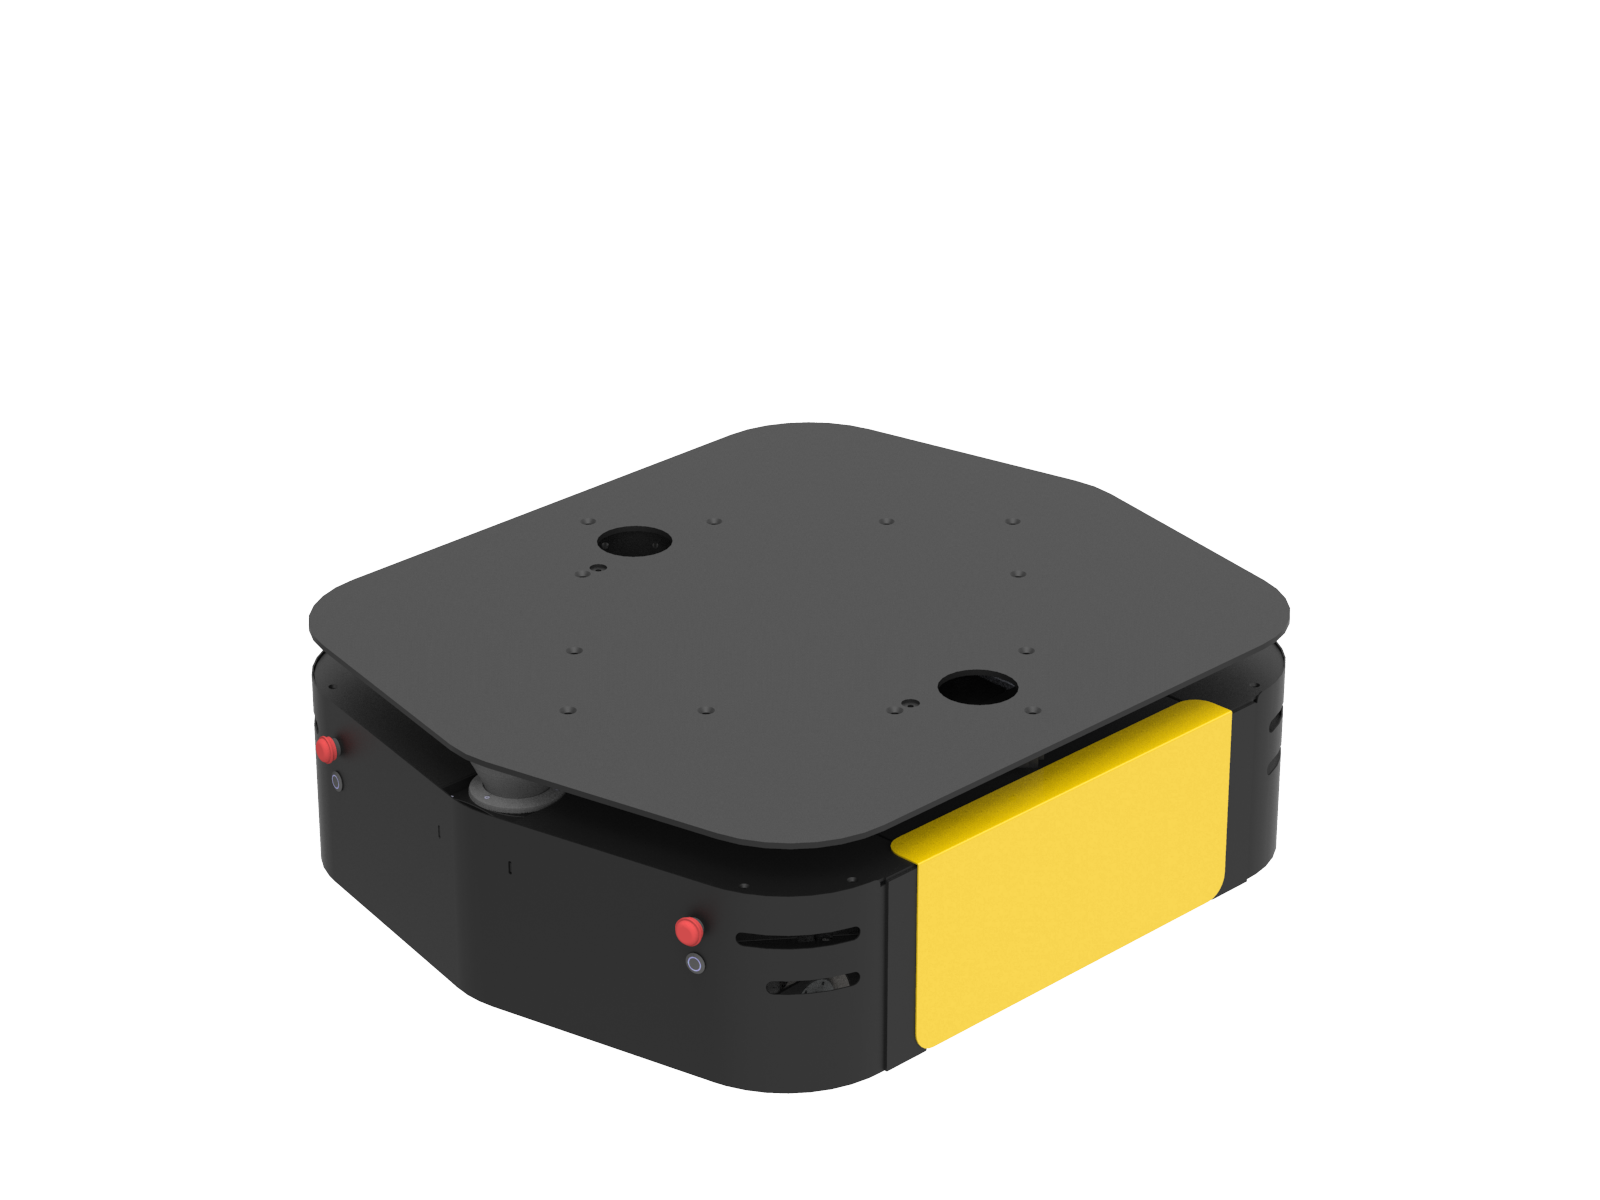
\includegraphics[width=0.75\textwidth]{images/ridgeback.png}
   \caption{Clearpath Ridgeback}
   \label{pics:ridgeback}
\end{figure}

\begin{table}[h]
\begin{center}
 \caption{Clearpath Ridgeback Specifications}\vspace{1ex}
 \label{tab:ridgeback}
 \begin{tabular}{ll}
 \hline
 Length & \unit[960]{mm}\\
 Width & \unit[793]{mm}\\
 Height & \unit[296]{mm}\\
 Weight & \unit[135]{kg}\\
 Maximum payload & \unit[100]{kg}\\
 Maximum velocity & \unitfrac[1.1]{m}{s}\\
 Average power consumption & \unit[800]{W}\\
 \hline
 \end{tabular}
\end{center}
\end{table}

The ridgeback is an omnidirectional robot platform designed by Clearpath for indoor movement and payload carrying tasks, such as autonomous warehousing for example. It is a fully integrated system with sensors, actuation and control and features a native ROS interface. Onboard sensors consist of an IMU and a front facing Hokuyo laser range finder (LIDAR) and a Kinect2 camera and wheel odometry. Optionally, a second, rear facing LIDAR can be mounted for full \unit[360]{\textdegree} coverage.The broad range of sensors, it's flexibility and low drift in odometry makes the Ridgeback a suitable and popular platform for research in controlled indoor environments.

Additionally, the Ridgeback houses the onboard computer that runs the low-level drivers of all the elements of the manipulator. On top thereof, there is a high-level driver that ensures accord and offers a ROS interface for the user to connect to.

\section{Universal Robot 10}

\begin{figure}
   \centering
   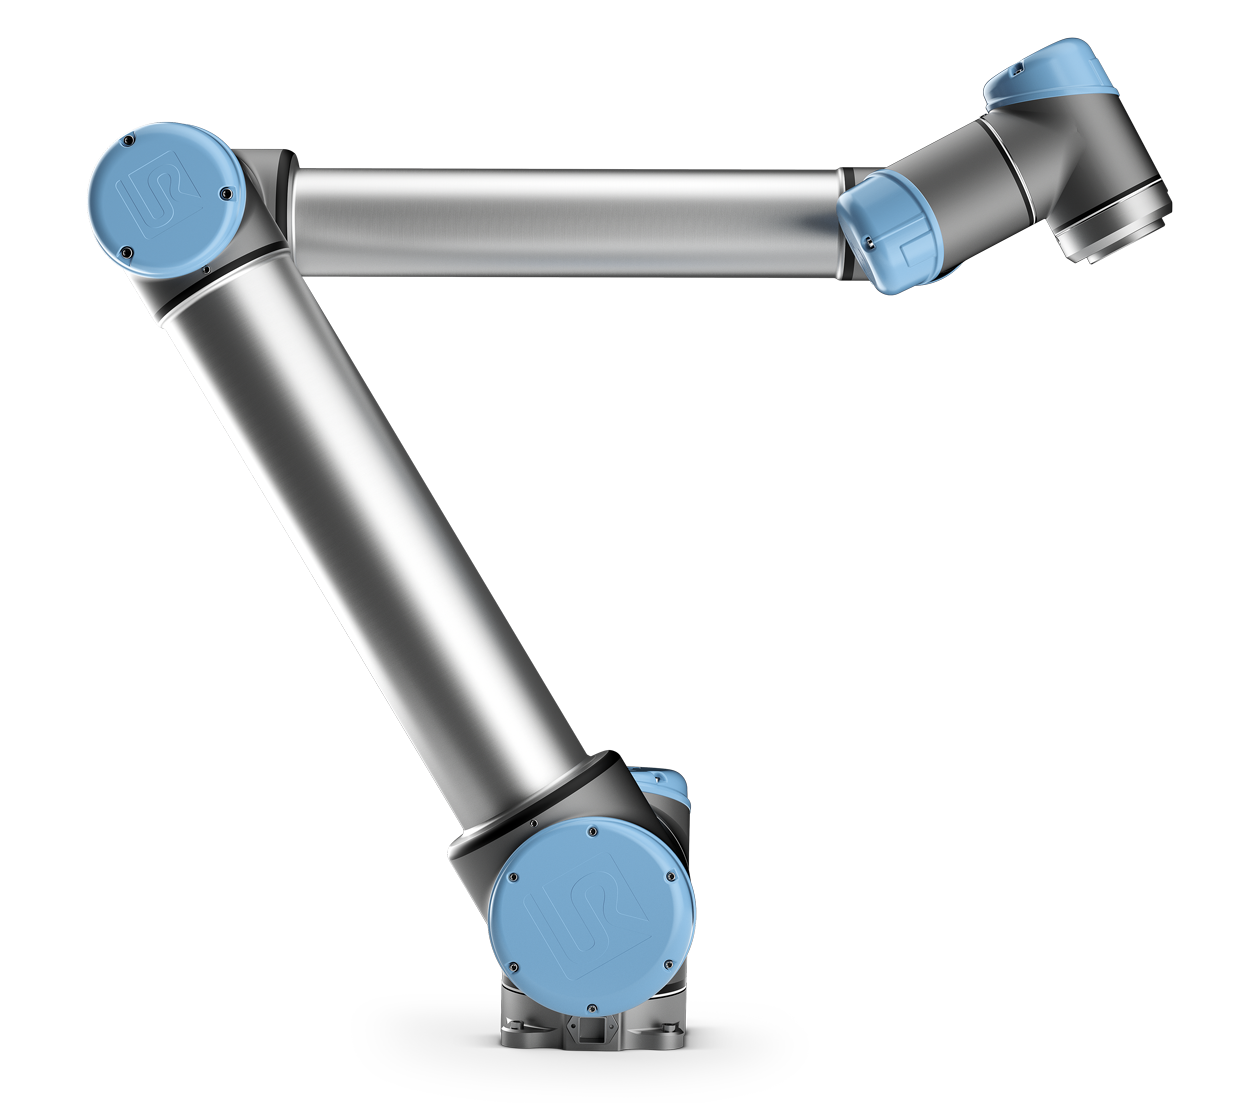
\includegraphics[width=0.75\textwidth]{images/ur10.png}
   \caption{Universal Robot 10}
   \label{pics:ur10}
\end{figure}

The UR10 is an collaborative industrial robot arm by Universal Robots. It has six rotary joints with gives it six DOF and can support payloads up to \unit[10]{kg}. Together with it's little brother the UR5, it is widely regarded as the standard manipulator within robotics research. Hence, extensive platform and software integration resources are available and ROS is supported out of the box.

\begin{table}[h]
\begin{center}
 \caption{Universal Robot 10 Specifications}\vspace{1ex}
 \label{tab:ur10}
 \begin{tabular}{ll}
 \hline
 Reach & \unit[1300]{mm} \\
 Weight & \unit[1.5]{kg}\\
 Repeatability & \unit[0.1]{mm} \\
 Maximum payload & \unit[10]{kg}\\
 Maximum tool velocity & \unitfrac[1]{m}{s}\\
 Degrees of freedom & 6 rotating joints \\
 Average power consumption & \unit[]{W}\\
 \hline
 \end{tabular}
\end{center}
\end{table}

\section{Gripper}

\begin{figure}
   \centering
   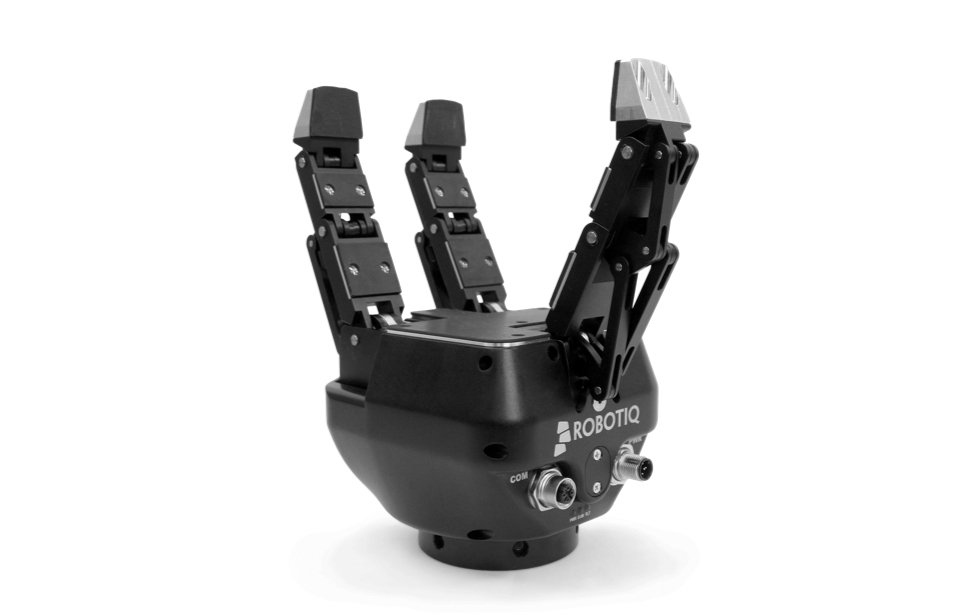
\includegraphics[width=0.75\textwidth]{images/robotiq_gripper.jpg}
   \caption{Robotiq 3-Finger Adaptive Robot Gripper}
   \label{pics:robotiq_gripper}
\end{figure}

\begin{table}[h]
\begin{center}
 \caption{Robotiq 3-Finger Adaptive Robot Gripper Specifications}\vspace{1ex}
 \label{tab:robotiq_gripper}
 \begin{tabular}{ll}
 \hline
 Weight & \unit[2.3]{kg}\\
 Repeatability & \unit[0.1]{mm} \\
 Maximum payload (encompassing grip) & \unit[10]{kg}\\
 Gripper opening & \unit[0 to 155]{mm} \\
 Object diameter for encompassing & \unit[20 to 155]{mm}\\
 Grip force & \unit[30 to 70]{N} \\
 Minimum power consumption & \unit[4.1]{W} \\
 Peak power (at maximum gripping force) & \unit[36]{W}\\
 \hline
 \end{tabular}
\end{center}
\end{table}

\section{Force-Torque Sensor}

\begin{figure}
   \centering
   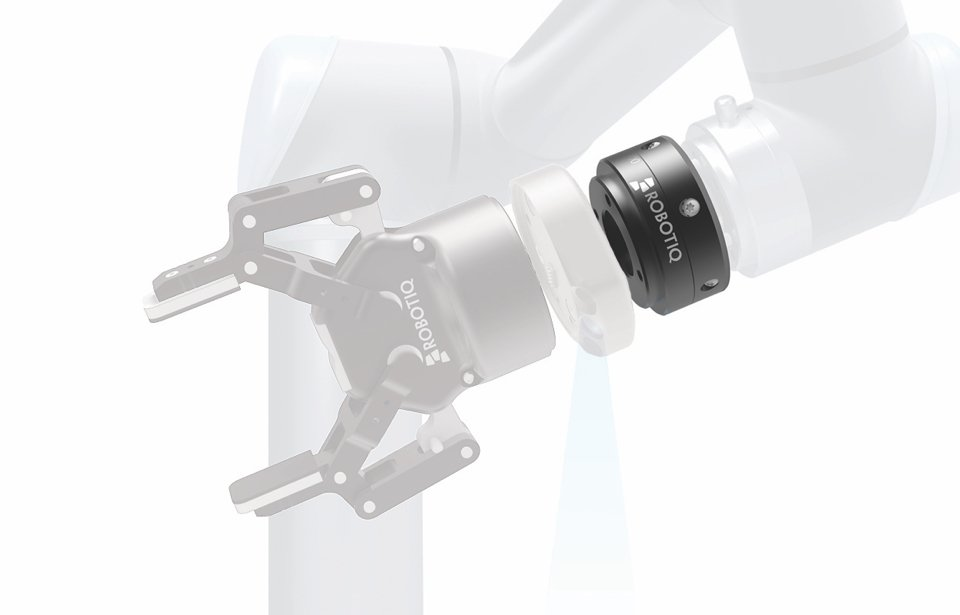
\includegraphics[width=0.75\textwidth]{images/robotiq_ft.jpg}
   \caption{Robotiq FT 300 Force Torque Sensor}
   \label{pics:robotiq_ft}
\end{figure}

\begin{savenotes}
\begin{table}[h]
\begin{center}
 \caption{Robotiq FT 300 Force Torque Sensor Specifications}\vspace{1ex}
 \label{tab:robotiq_ft}
 \begin{tabular}{ll}
 \hline
 \textbf{Measuring range} & \\
 Force $F_x, F_y, F_z$ & \unit[$\pm 300$]{N} \\
 Moment $M_x, M_y, M_z$ & \unit[$\pm 30$]{Nm} \\ \hline
 \textbf{Signal noise}\footnote{Signal noise is the standard deviation of the signal measured over a period of one second.} &\\
 Force $F_x, F_y, F_z$ & \unit[0.1]{N} / \unit[1]{N} \\
 Moment $M_x, M_y$ & \unit[0.05]{Nm} / \unit[0.02]{Nm} \\
 Moment $M_z$ & \unit[0.03]{Nm} / \unit[0.01]{Nm} \\ \hline
 Data output rate & \unit[100]{Hz} \\
 Weight & \unit[300]{g}\\
 \hline
 \end{tabular}
\end{center}
\end{table}
\end{savenotes}


\chapter{Admittance Control}
The term admittance is closely coupled to impedance \citep{hogan1985impedance}.


\chapter{Obstacle Avoidance}
Ever since robots faced the task of autonomous navigation, obstacle avoidance has been a crucial element of it. There are numerous approaches to tackle the problem, varying in degrees of foresight and influence on the path planner.

The problem can be seperated into two categories, path planning on a global scale and on a local scale. The first category bundles algorithms that take a goal position and a current position of a robot and calculate the optimal path (usually the shortest path) in between, given some objective function. Since the distance to the goal is normally greater than the range of any obstacle detection sensor, these algorithms need a full map of the environment. Widely used examples are A*, Djikstra, Bit* and RRT.

In contrast, path planning on a local scale takes obstacle detection sensor information as an input and outputs commands to a drive unit, that meet the given objective, which is usually to avoid collisions and stay clear of an obstacle by a minimum distance. 

A typical path planning infastructure on a robot consists of both a global and a local planner, where the global planner outputs a path to follow to the local planner, which in terms fuses that path with online obstacle detection sensor information to ensure it is indeed collision free and deviates from it if necessary.

To find the path planning algorithm that best meets our needs, we must first examine what are the given inputs and the desired outputs of our system. As we already elaborated in \cref{sec:introduction}, we are working in a classical master-slave scenario, which means that the robot is trying to achieve the goal of its human counterpart and not its own. This manifests in the planner in such a way, that the input is the force and torque applied by the human and the robot has no global goal pose. Hence, we are inherently bound to iteratively updated goals within close proximity and there is no possibility nor need to apply global path planning techniqes and we focus only on local planners in the remainder of this chapter.

\section{Local Planners}
In this chapter, we discuss a selection of common local planning methods and their feasibility for the task at hand.
\subsection{Velocity Obstacles}
Velocity Obstacles (VO) \citep{fiorini1998motion}

\begin{equation}
p_{RO} + v_R t < r_R +r_O
	\label{eq:vo_condition}
\end{equation}

\begin{equation}
VO_{RO} = D TODO fill in
\end{equation}
\subsection{Dynamic Window Approach}
The Dynamic Window Approach (DWA) \citep{fox1997dynamic} is a well-known algorithm that produces command velocities for a planar robot given vehicle dynamics and obstacle measurements. The basic assumption is that the robot moves instantaneously on circular arcs with a translational velocity $v$ and a rotational velocity $\omega$. Thus, the complexity is greatly simplified and calculations are be performed in the 2D velocity space $(v,\omega)$. Within this space, we compute three sets of velocity pairs,  subsequently called \emph{windows} for every iteration of the algorithm.

The \emph{obstacle window} $V_o$ are the measurements of any obstacles, e.g. taken by a range laser sensor and transformed from cartesian to $v,\omega$ space.

The \emph{static window} $V_s$ expresses the constraint velocities of the vehicle, i.e., absolute maximum and minimum velocity. As the name suggests, these parameters are usually static and do not need to be recalculated every step.

The \emph{dynamic window} $V_d$ are the vehicle dynamics, i.e., velocities that are physically feasible for the robot to reach within one timestep. It's size is defined by the maximal acceleration and the current velocity of the robot.

\begin{equation}
V_r = V_o \cap V_s \cap V_d
 	\label{eq:dwa_intersection}
\end{equation}

As \cref{eq:dwa_intersection} shows, the intersection of these three sets gives us the resulting window $V_r$ of feasible velocity pairs, that guarantee no collision with an obstacle for the next step.

A cost function is then applied to find the $(v,\omega)$ pair, that maximizes the objective within $V_r$. Elements are heading, distance to goal and velocity terms.

\subsection{Potential Fields}
Potential fields are also a common tool in the mobile robotics field used for path planning. A virtual potential $U(q)$ at position $q = (x,y)$ affects the robot and drives him away from any maximum, like a ball rolling downhill \citep{siegwart2004autonomous}. It can be used to attract the robot to a goal by creating a local minimum and repulsing a robot from an obstacle by creating a local maximum.

If the potential field is differentiable, we find that the resulting virtual force $F(q)$ that acts on the robot in position $q$ is then defined as 
\begin{equation}
F(q) = - \nabla U(q) 
	\label{eq:pot_force}
\end{equation}
where $\nabla U(q)$ is the gradient of the potential field
\begin{equation}
\nabla U(q) = \begin{pmatrix}
\frac{\partial U}{\partial x}
\frac{\partial U}{\partial y}
\end{pmatrix}
\end{equation}


The overall potential field is the sum of all attractive and repulsive potential fields
\begin{equation}
U(q) = U_{attr}(q) + U_{rep}(q)
	\label{eq:pot_field}
\end{equation}
and by combining \ref{eq:pot_force} and \ref{eq:pot_field} we see the virtual force consists of:
\begin{equation}
\begin{aligned}
F(q) &= F_{att}(q) + F_{rep}(q) \\
&= -\nabla U_{att}(q)-\nabla U_{rep}(q)
\end{aligned}
\end{equation}


An \textbf{attractive potential}, i.e. a goal is usually defined as a parabolic function

\begin{equation}
U_{att}(q) = \frac{1}{2} k_{att} \cdot {\rho_{goal}}^2(q)
\end{equation}

where $k_{att}$ is the scaling factor and $\rho_{goal}$ is the Euclidian distance to the goal:
\begin{equation}
\rho_{goal} = ||q-q_{goal}||
\end{equation}


A \textbf{repulsive potential}, i.e. an obstacle is zero if a certain distance is exceeded and should rise drastically when the robot gets within close proximity of the obstacle. Hence, a common definition is
\begin{equation}
U_{rep}(q) = \begin{cases}
      \frac{1}{2} k_{rep}\cdot (\frac{1}{\rho (q)}-\frac{1}{\rho_0})^2 & \text{if}\ \rho (q) \leq \rho_0 \\
      0 & \text{if}\ \rho (q) \geq \rho_0 \\
    \end{cases}
\end{equation}
where $k_{rep}$ is the scaling factor, $\rho_0$ is the distance threshold and $\rho (q)$ is the minimal distance from position $q$ to the obstacle.


The main limitation to this approach is that it is prone to local minima, where the robot can get stuck. However, we are not working with any goals, but rather with an user input in form of a force so even if the robot is within a local minima, the user can literally pull it away from it. Furthermore, because the output of the potential field method is a force vector, we can elegantly combine it with the admittance controller, which also operates using virtual forces acting on the robot. 

So we can conclude that the potential field method is most suitable for a fusion with an admittance controller and we will elaborate on our implementation in the following.

\chapter{Implementation}
\begin{figure}
   \centering
   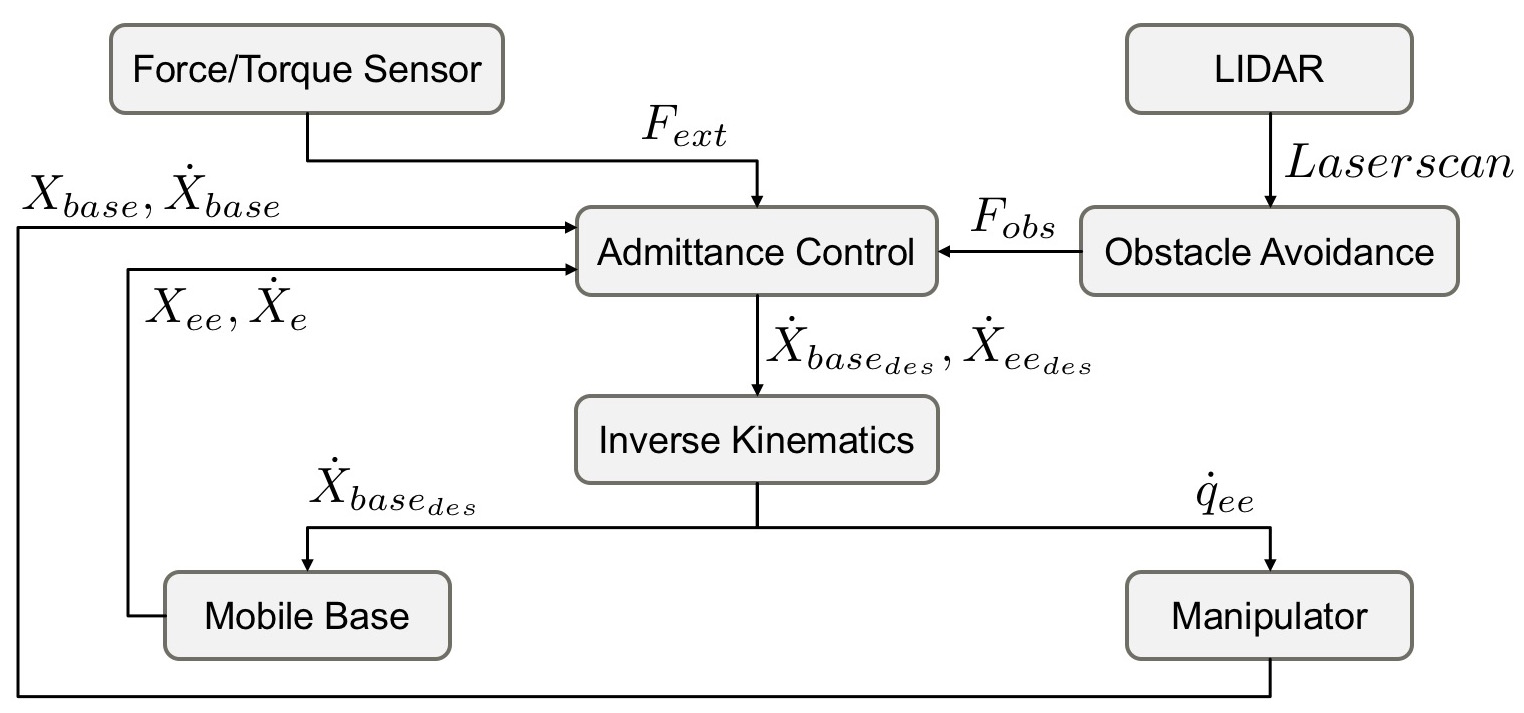
\includegraphics[width=0.75\textwidth]{images/controller_overview.jpg}
   \caption{Schematic of the controller. Arrows indicate information flow between the subsets of the control architecture.}
   \label{pics:controller_overview}
\end{figure}

Flowchart of the whole algorithm comes here
\section{Admittance Control and Obstacle Avoidance Fusion}
\begin{figure}
   \centering
   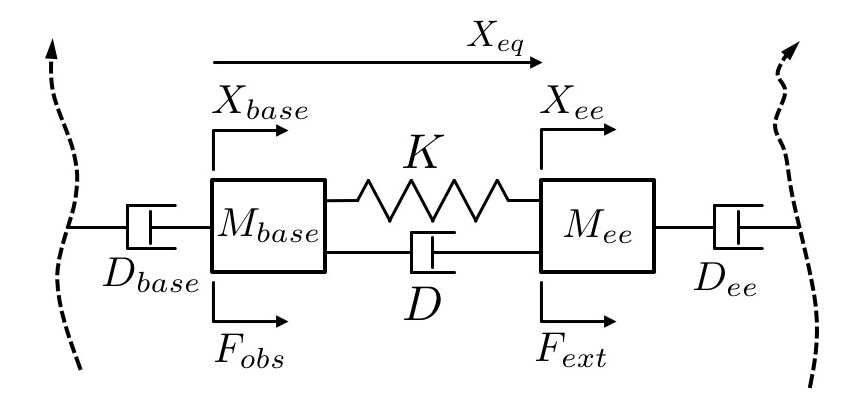
\includegraphics[width=0.75\textwidth]{images/admittance_model.jpg}
   \caption{Virtual spring mass damper system with two masses. Dotted arrows represent the path of the base (left) and the arm (right) over time, connected by the spring mass damper system.}
   \label{pics:admittance_model}
\end{figure}


\subsection{Parameters}
admittance parameters
\subsection{Costmap}
\begin{figure}
   \centering
   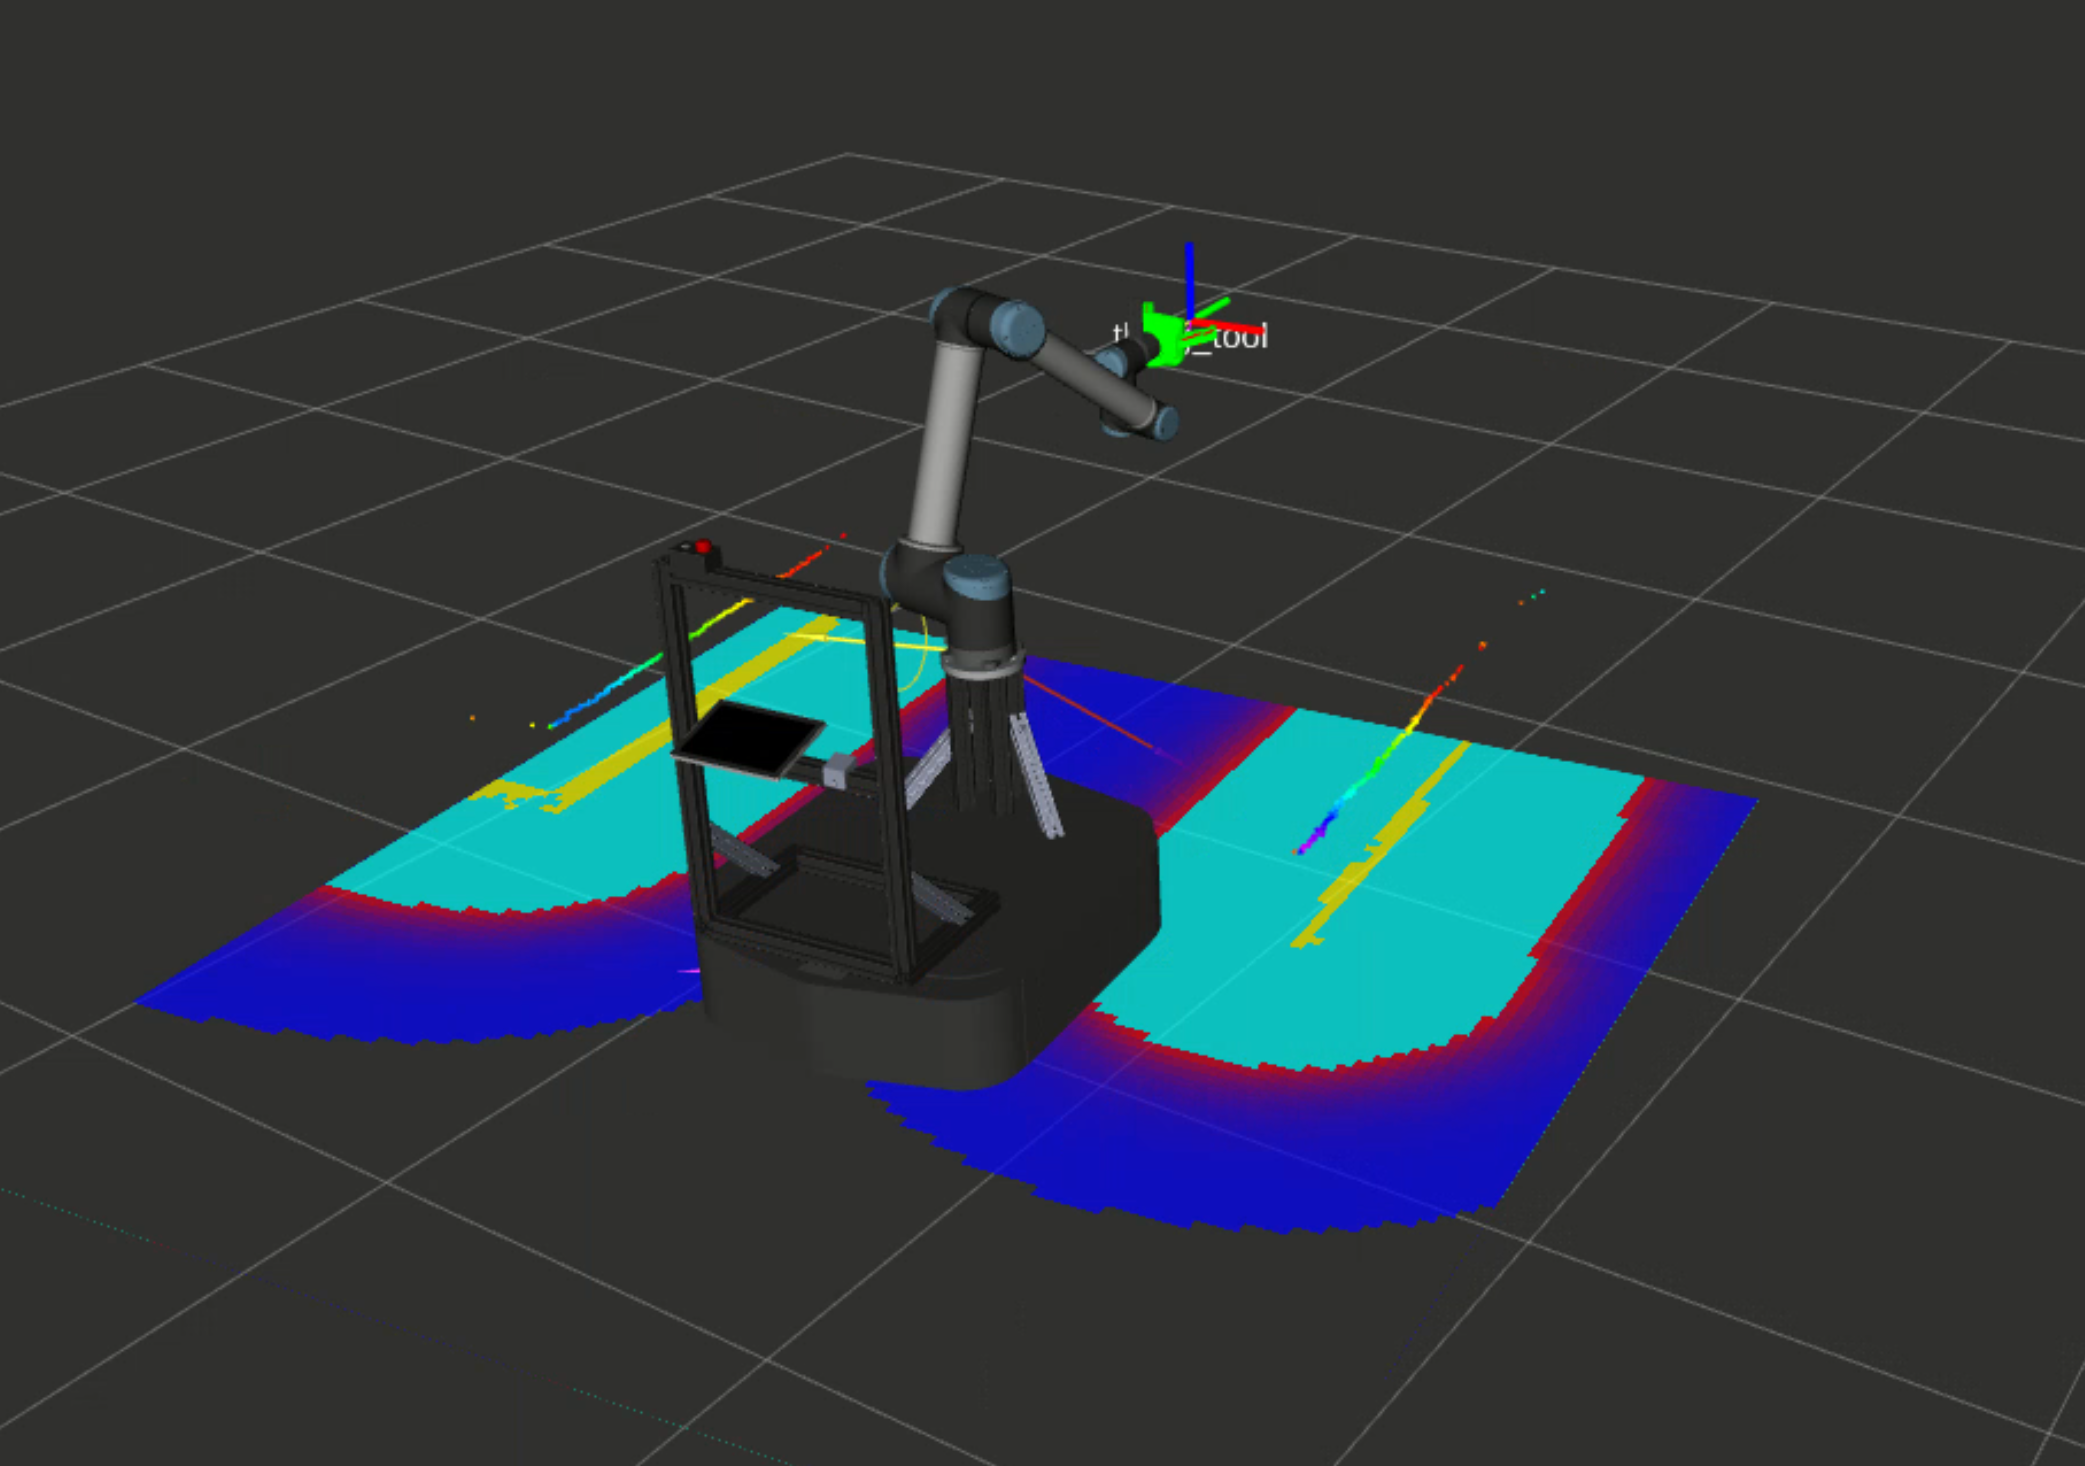
\includegraphics[width=0.75\textwidth]{images/costmap.png}
   \caption{Costmap captured by the LIDAR during a test. YELLOW: Lethal, TURQUOISE: Inscribed, RED TO BLUE GRADIENT: Proximity to an obstacle, TRANSPARENT: Free space. }
   \label{pics:costmap}
\end{figure}

\begin{description}
  \item[Lethal] dini 
  \item[Inscribed] sini
  \item[Obstacle proximity]
  \item[Freespace]
\end{description}

\begin{table}[h]
\begin{center}
 \caption{Costmap Parameters.}\vspace{1ex}
 \label{tab:costmap_params}
 \begin{tabular}{ll}
 \hline
Type & Local \\
Update frequency & \unit{60}{Hz} \\
Publish frequency & \unit{60}{Hz} \\ 
Width & \unit{3}{m} \\
Height & \unit{3}{m} \\
Resolution & \unit{0.03}{m} \\
Global frame & Base link \\
Static map & False \\
Rolling window & True \\
Robot footprint & \unit{0.96 $\times$ 0.8}{m} \\
Plugins used & Obstacles layer, inflater layer \\
Inflater layer cost scaling factor & 10  \\
Inflation radius & \unit{2}{m} \\
 \hline
 \end{tabular}
\end{center}
\end{table}

\section{Inverse Kinematics}
task priority solver (parameters?)
\chapter{Results}
We test the implementation of the previously elaborated algorithm on the Thing and list the performed tests and their results in this chapter.
\section{Admittance Control Performance}
Before any experiments on the fused algorithm can be performed, we first analyze the behaviour of the admittance controller in isolation. For this, we place the Thing in free space, i.e., in a a region with zero gradient and wegerregen the the three axes of the ridgeback seperately.

\subsection{Force Excitement in X}
\begin{figure}
   \centering
   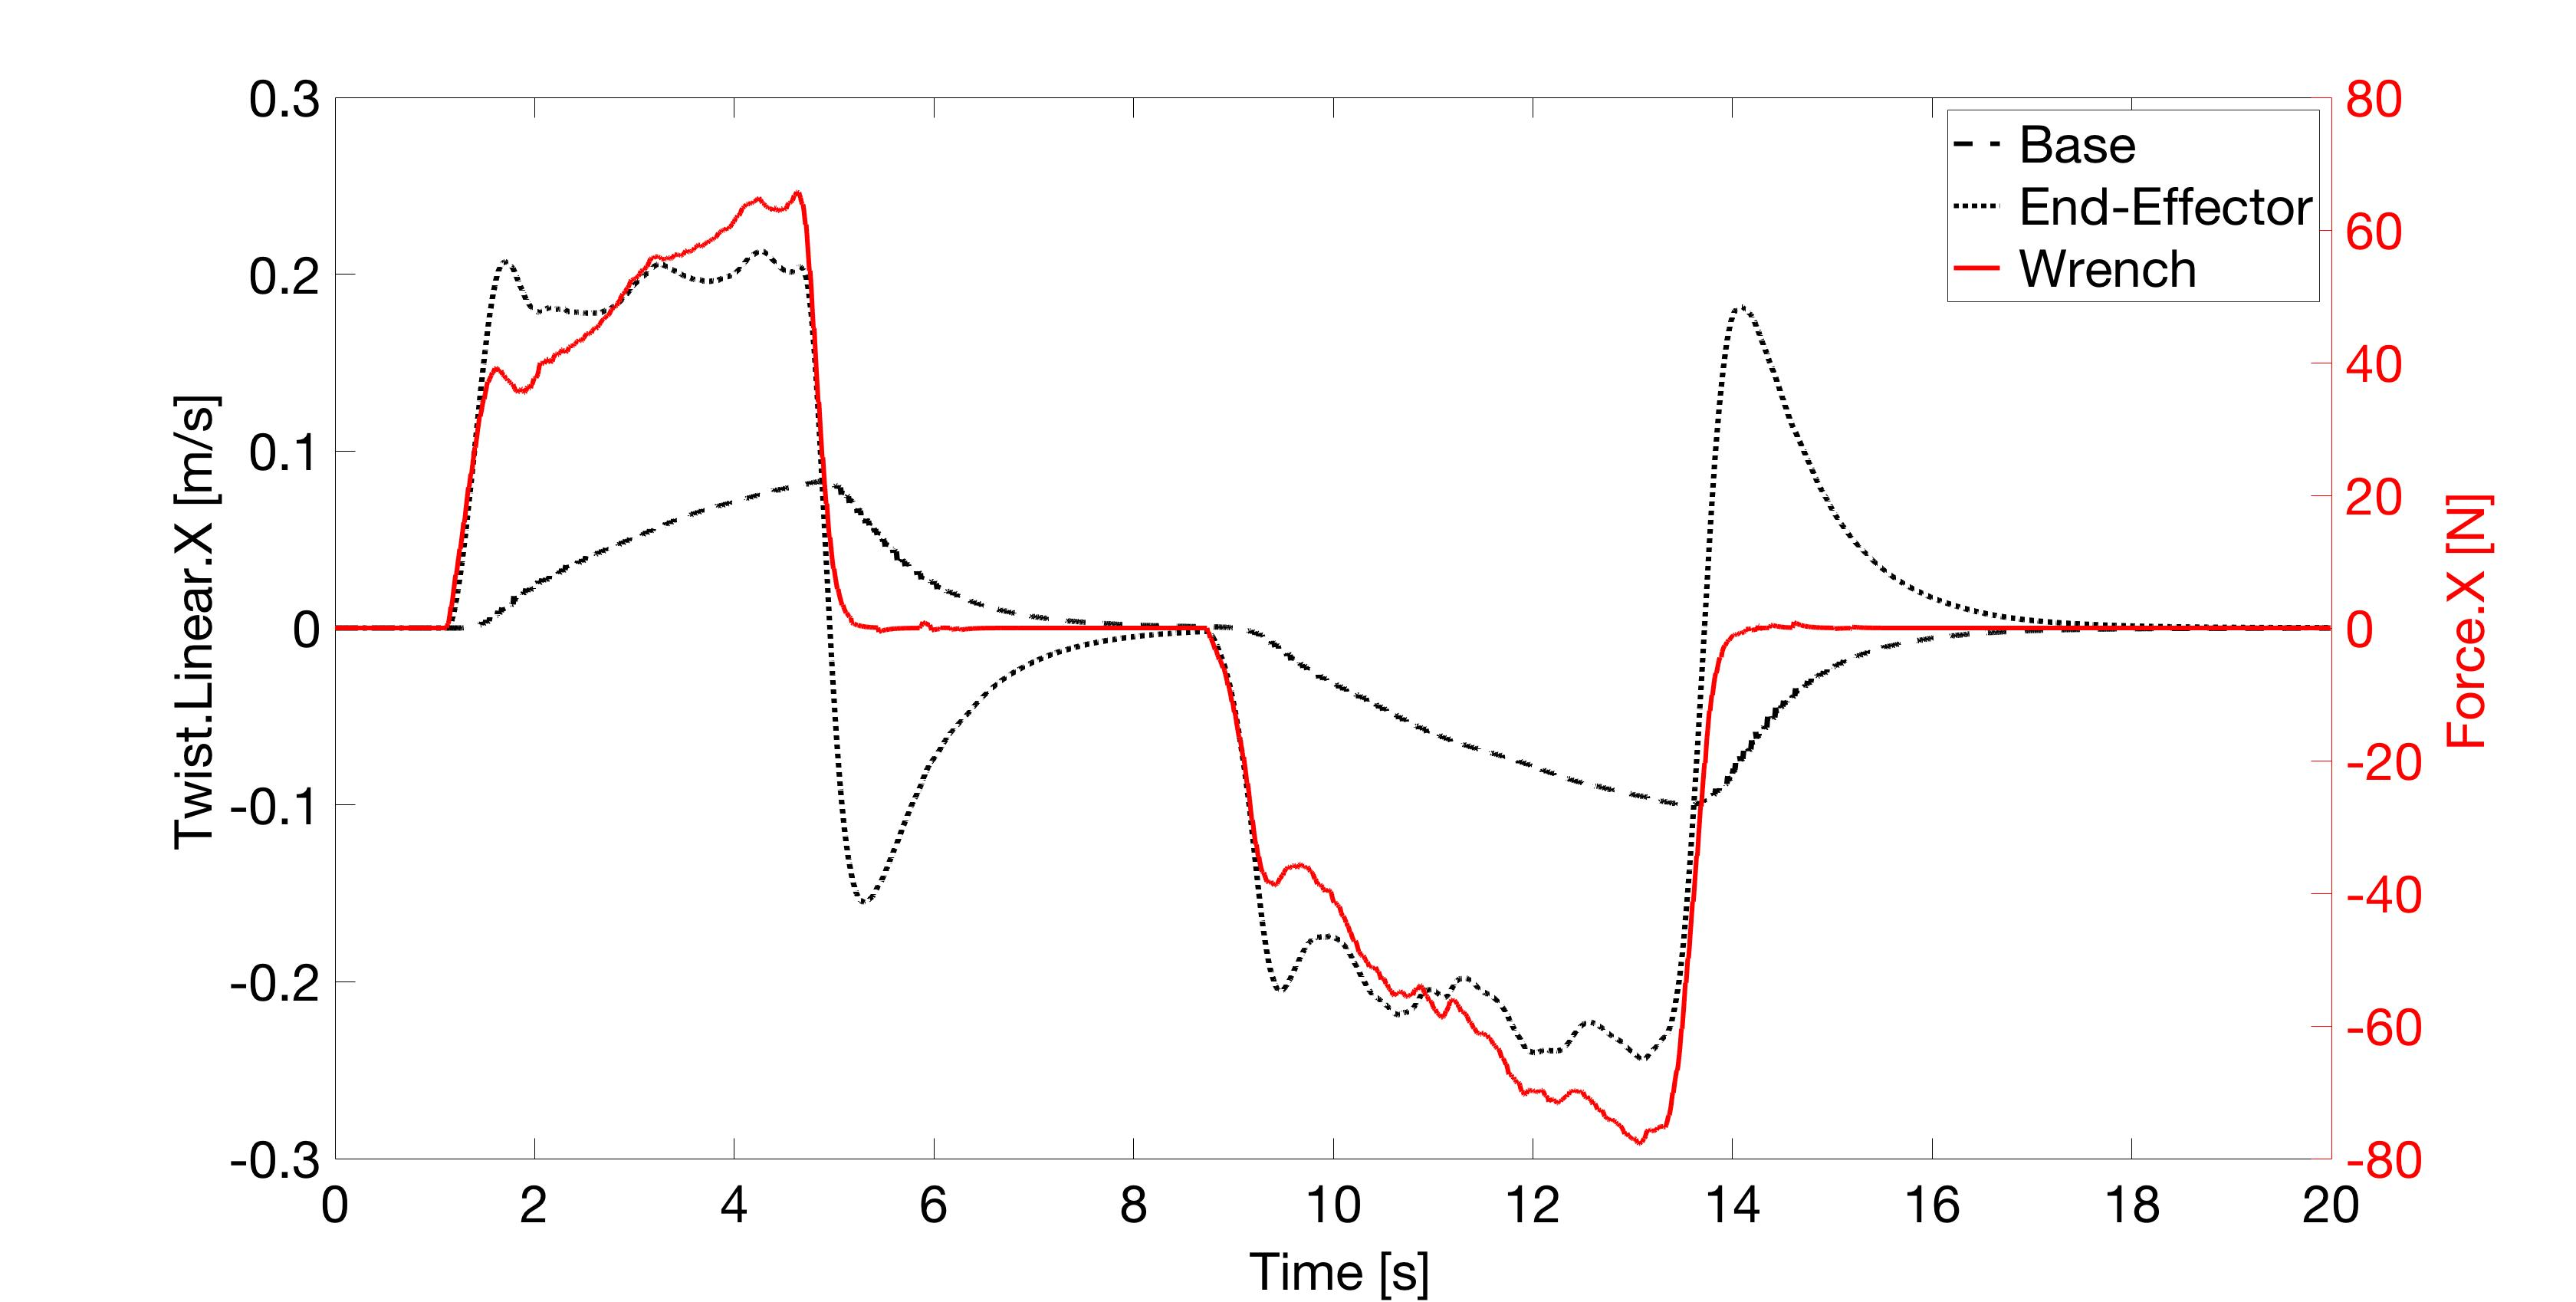
\includegraphics[width=0.75\textwidth]{images/test18_x.jpg}
   \caption{Velocity Response to Force Excitement in X}
   \label{pics:test18_x}
\end{figure}

\subsection{Force Excitement in Y}
\begin{figure}
   \centering
   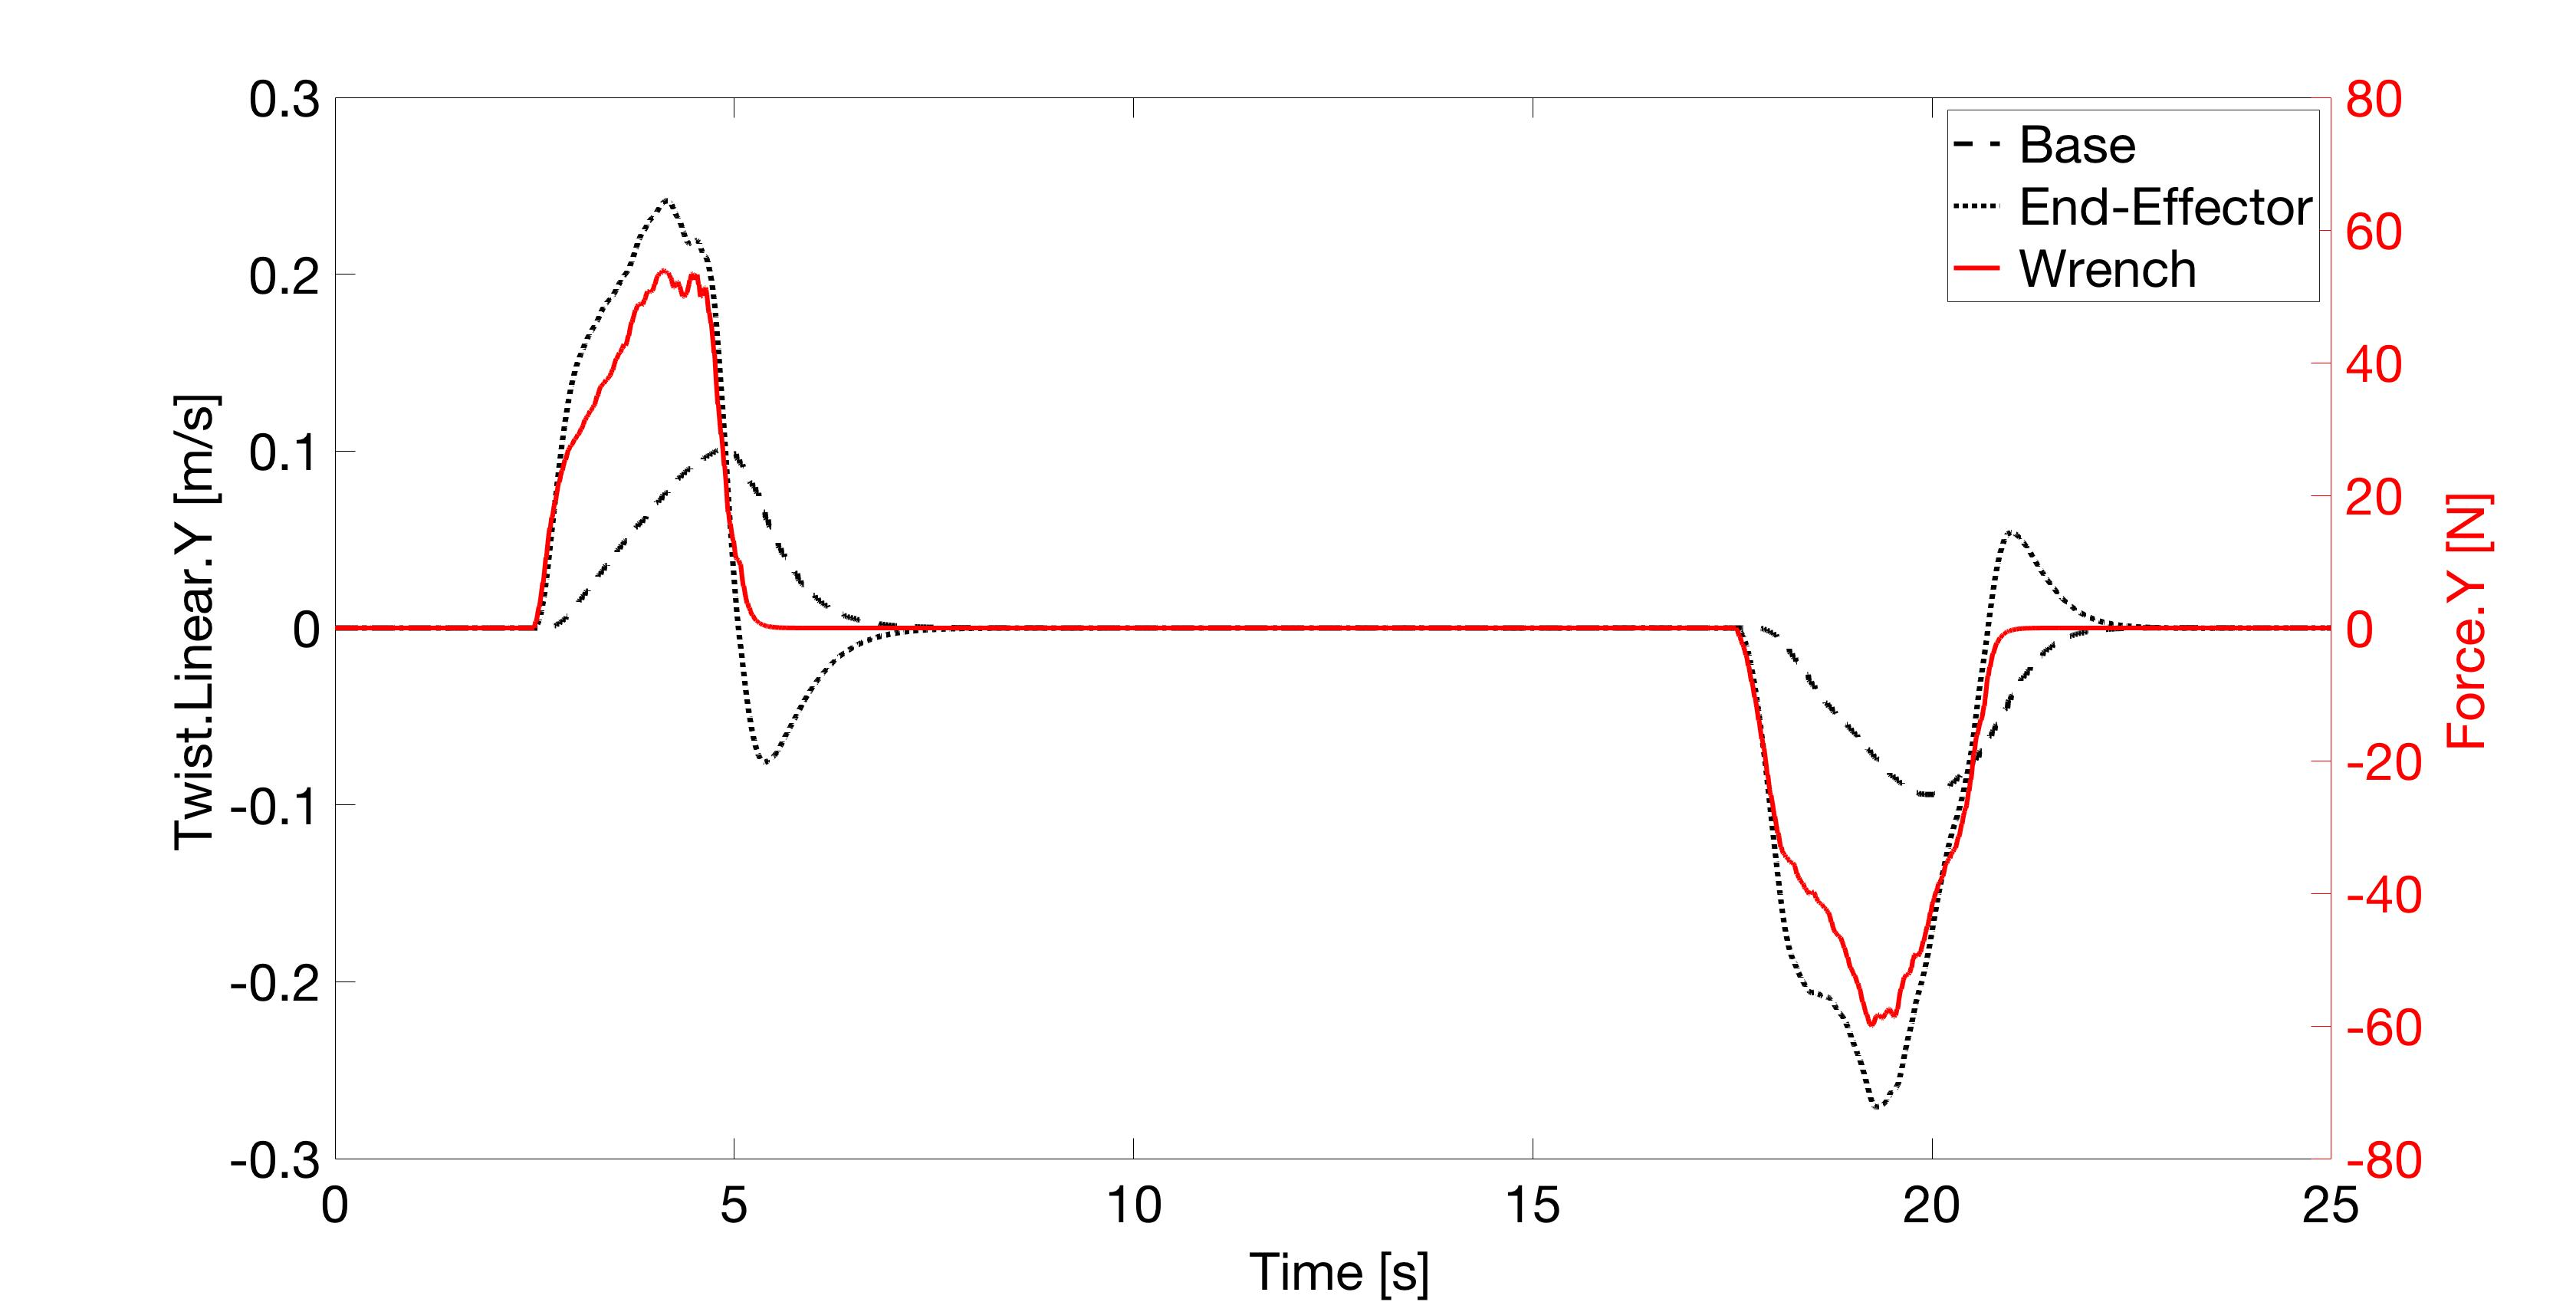
\includegraphics[width=0.75\textwidth]{images/test18_y.jpg}
   \caption{Velocity Response to Force Excitement in Y}
   \label{pics:test18_y}
\end{figure}
\subsection{Force Excitement in Theta}
\begin{figure}
   \centering
   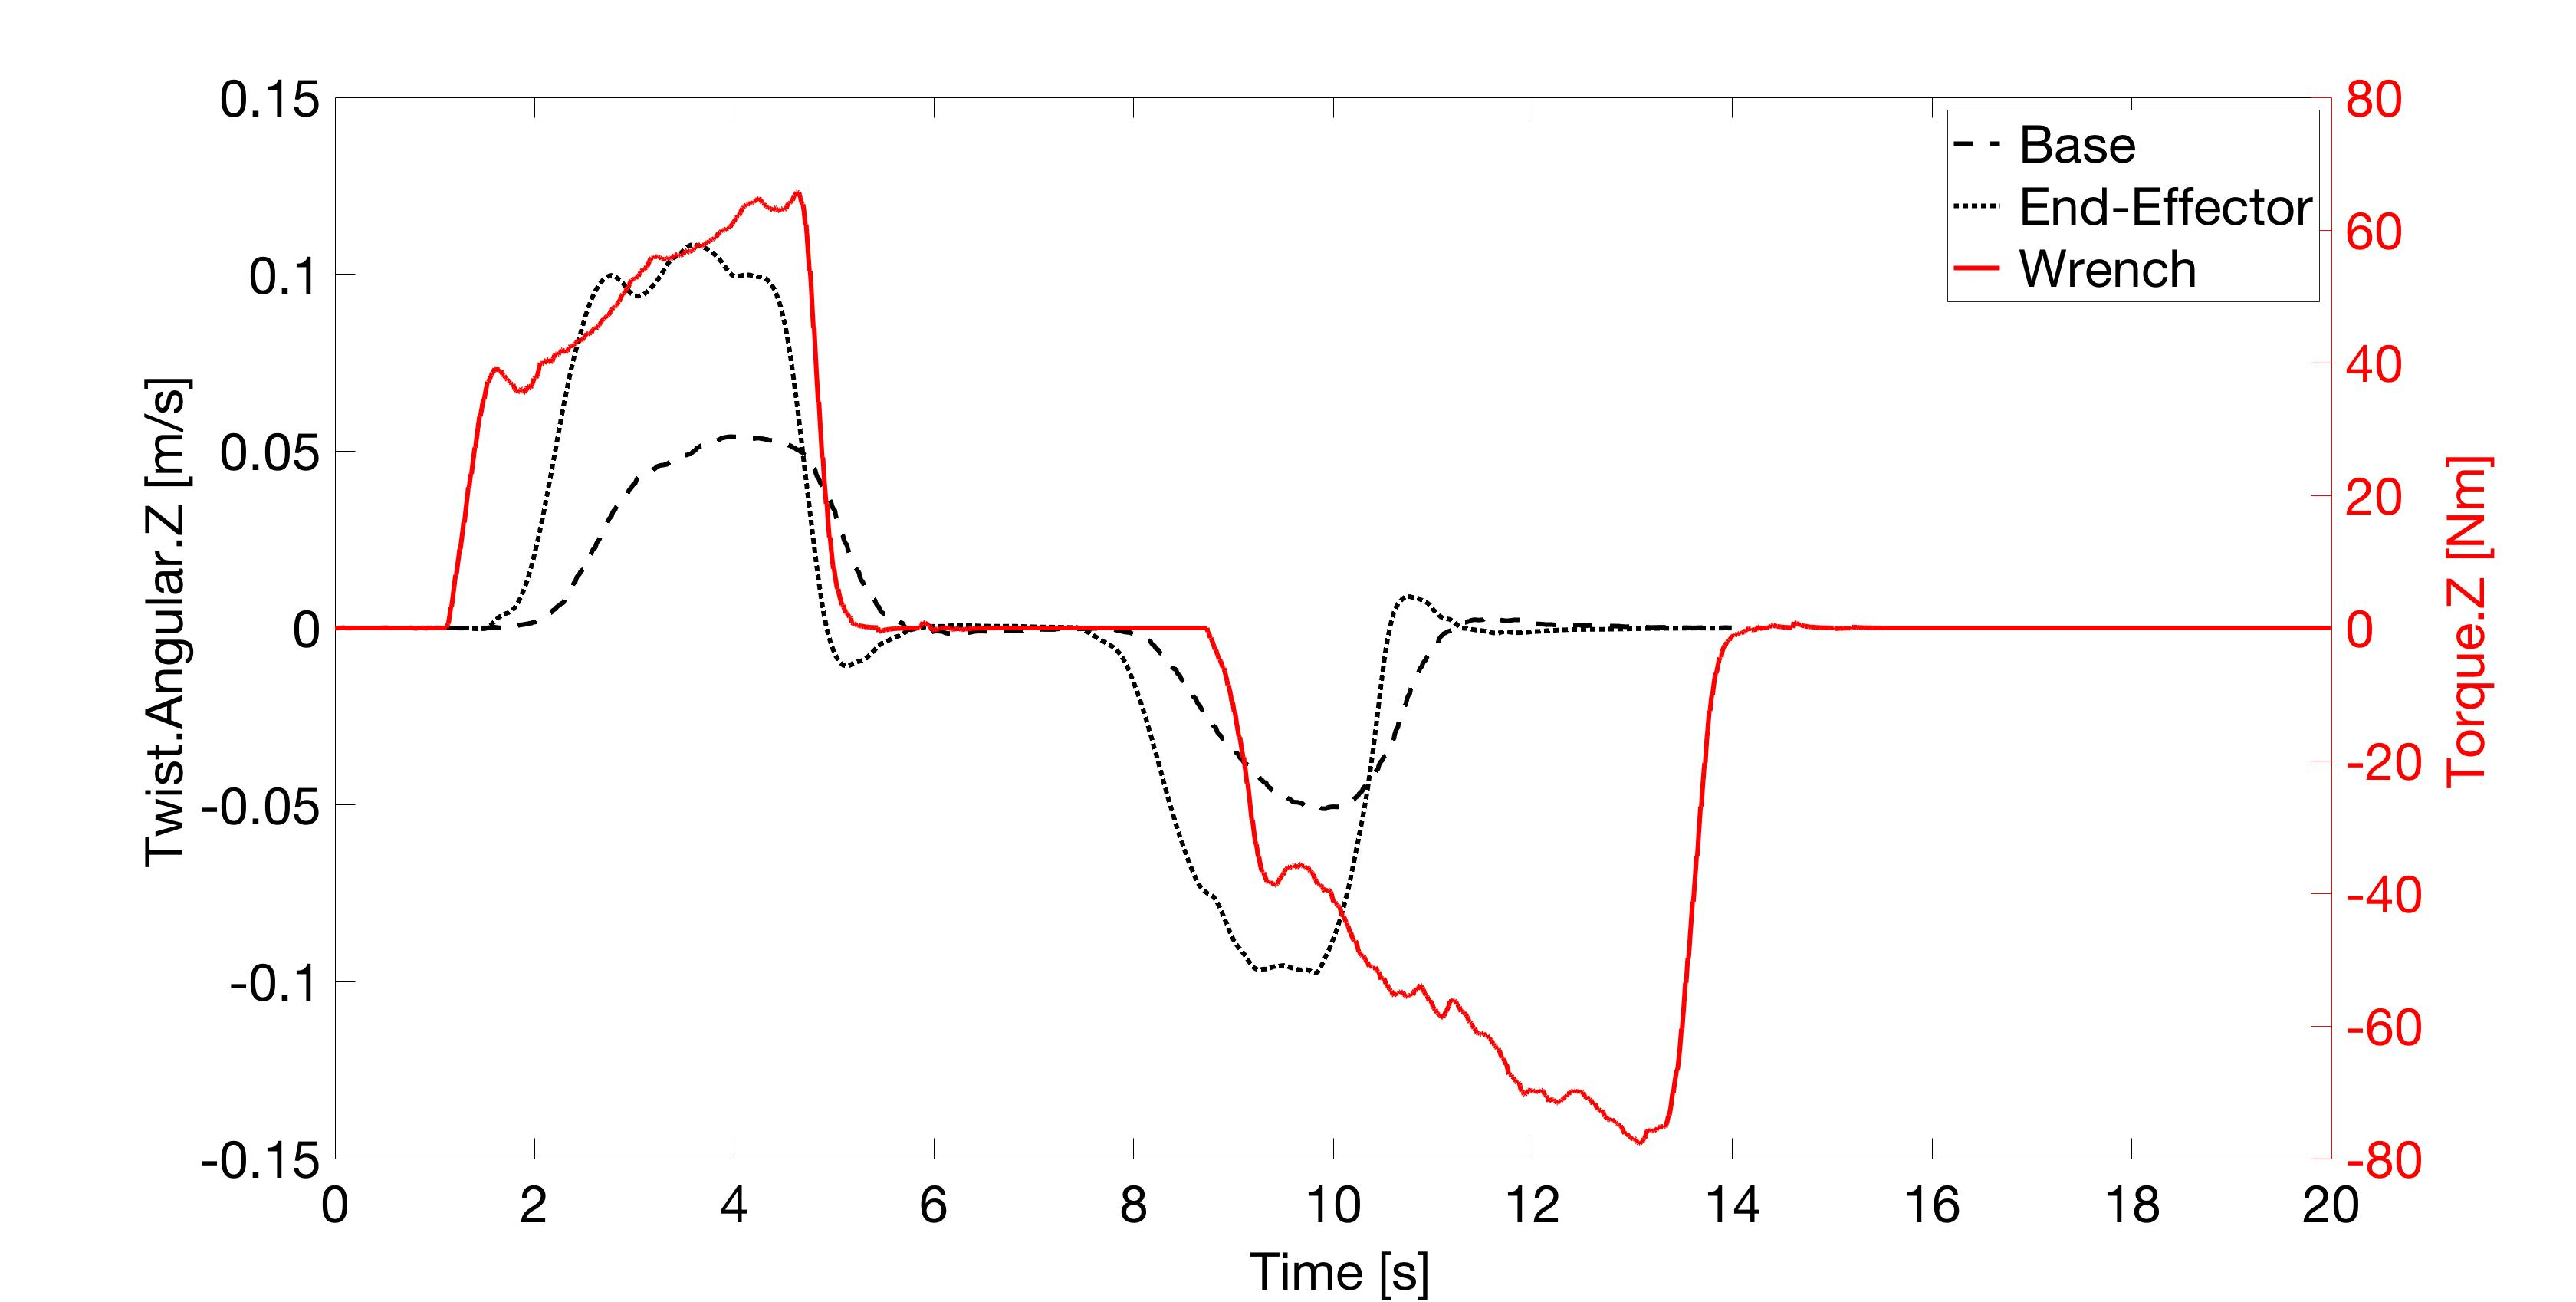
\includegraphics[width=0.75\textwidth]{images/test18_theta.jpg}
   \caption{Velocity Response to Force Excitement in $\theta$}
   \label{pics:test18_theta}
\end{figure}

\section{Obstacle Avoidance Performance}
\subsection{Frontal Obstacle}
\begin{figure}
   \centering
   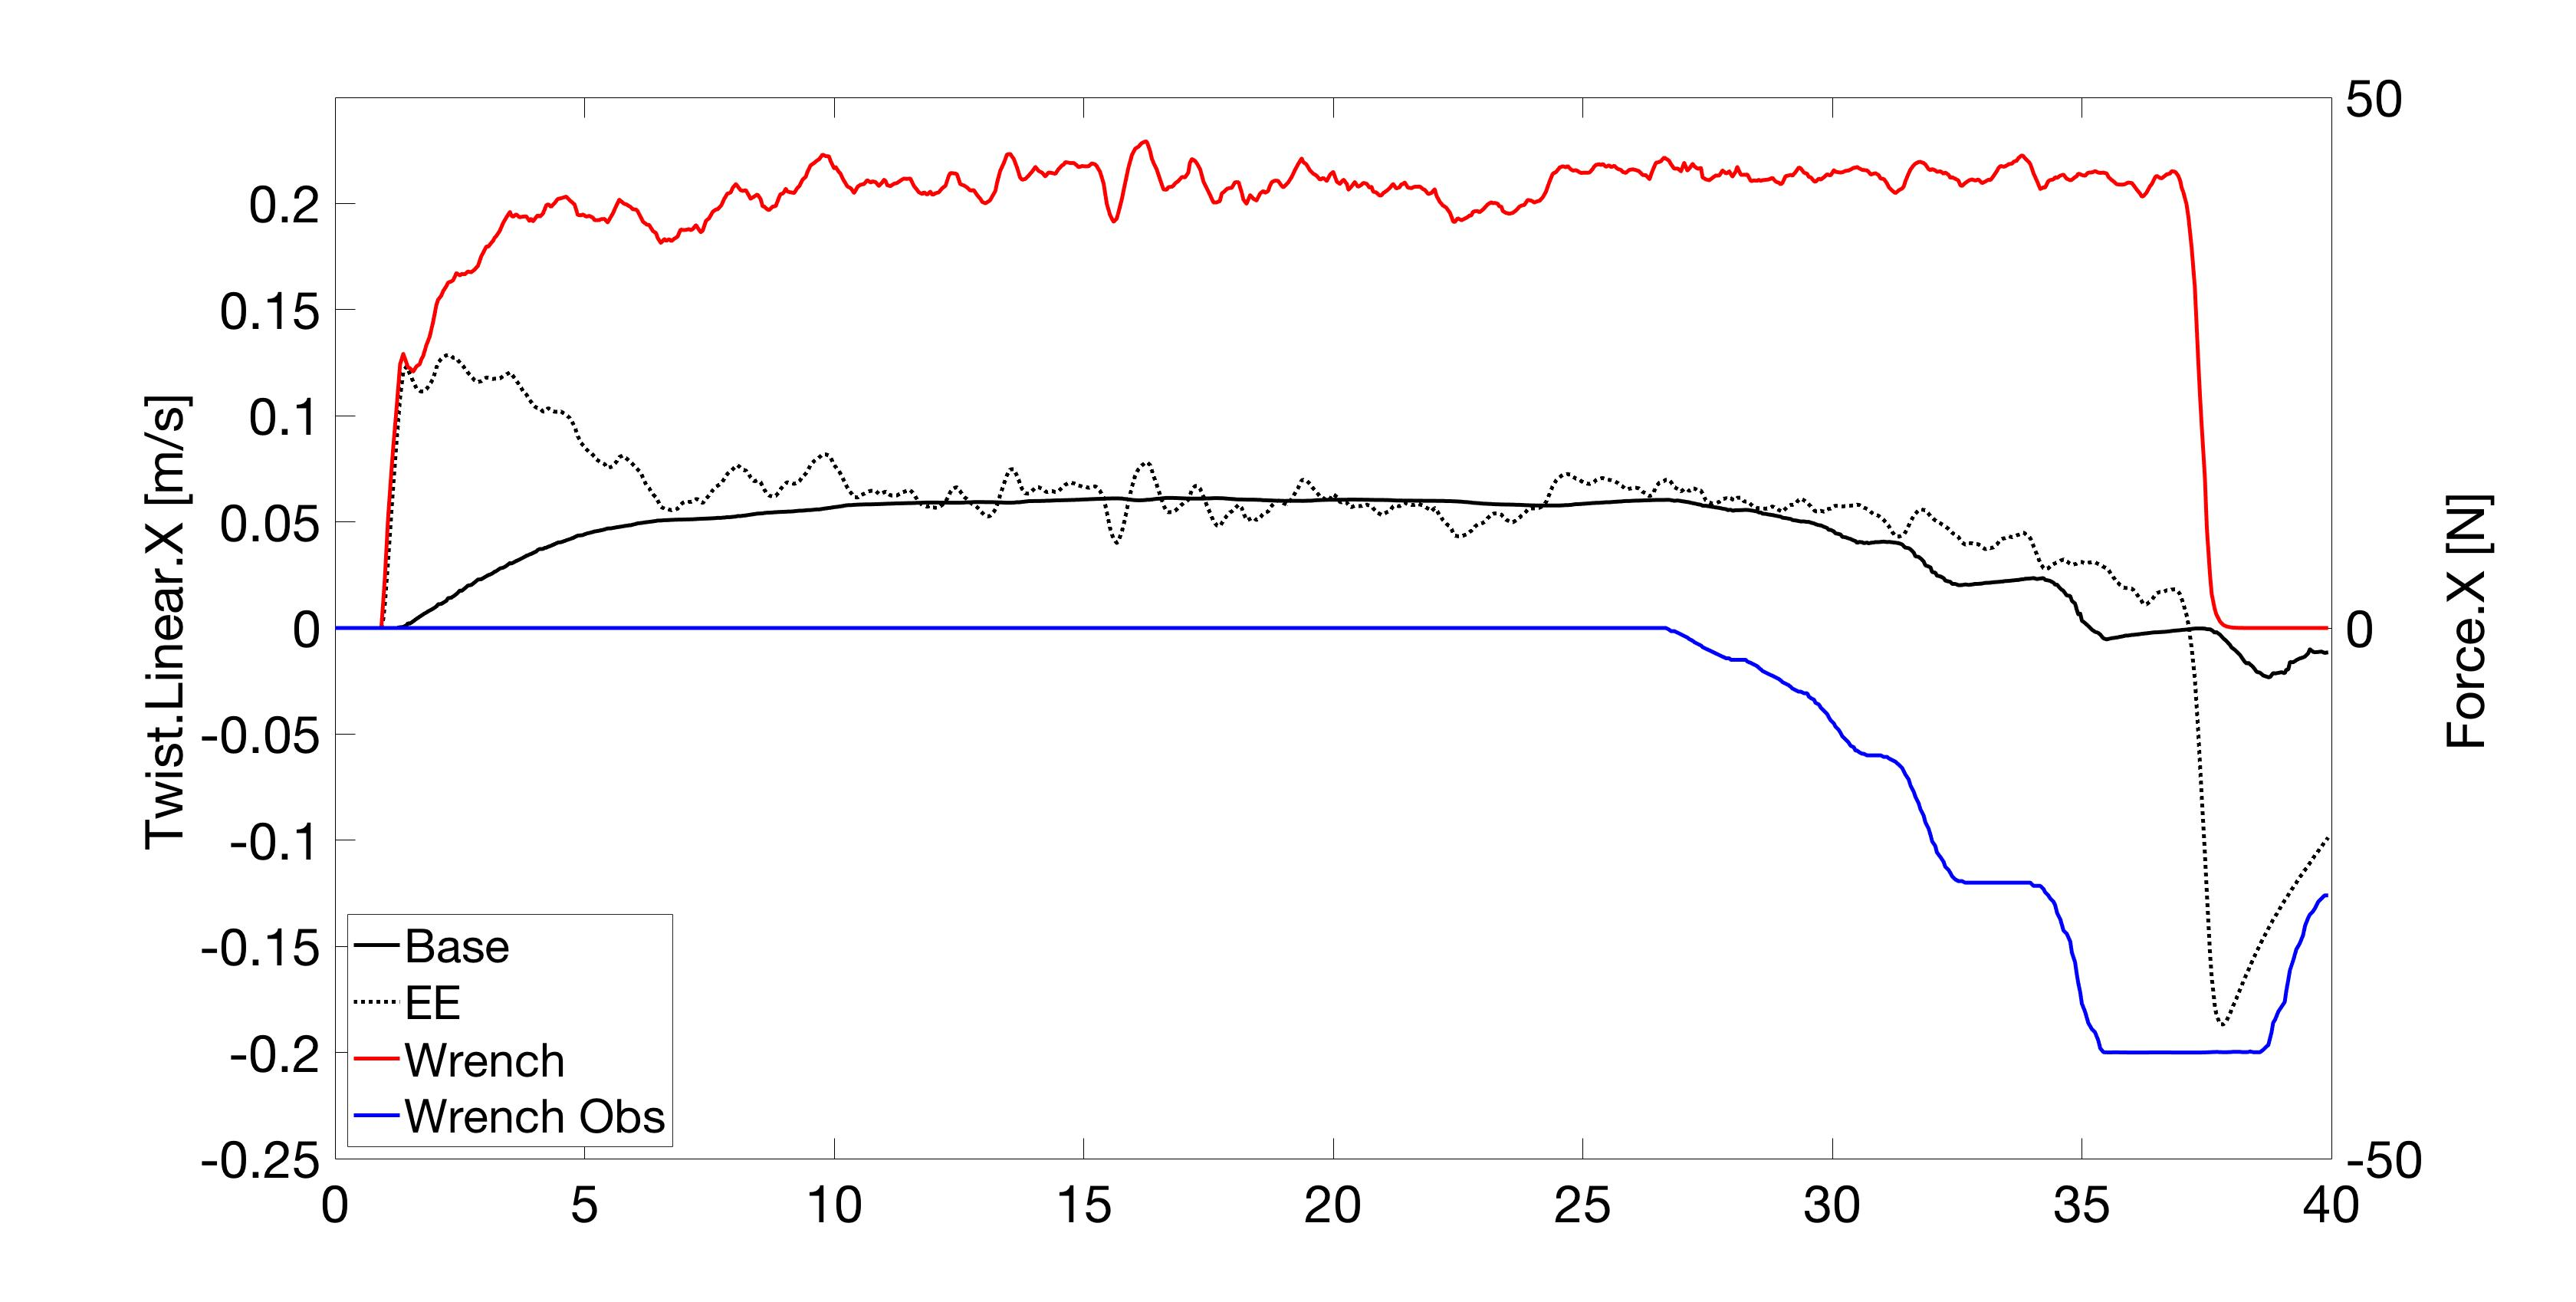
\includegraphics[width=0.75\textwidth]{images/test2.jpg}
   \caption{Velocity response in X axis of the robot to external and obstacle force input while being pulled in a frontal obstacle.}
   \label{pics:test2}
\end{figure}

\begin{figure}
   \centering
   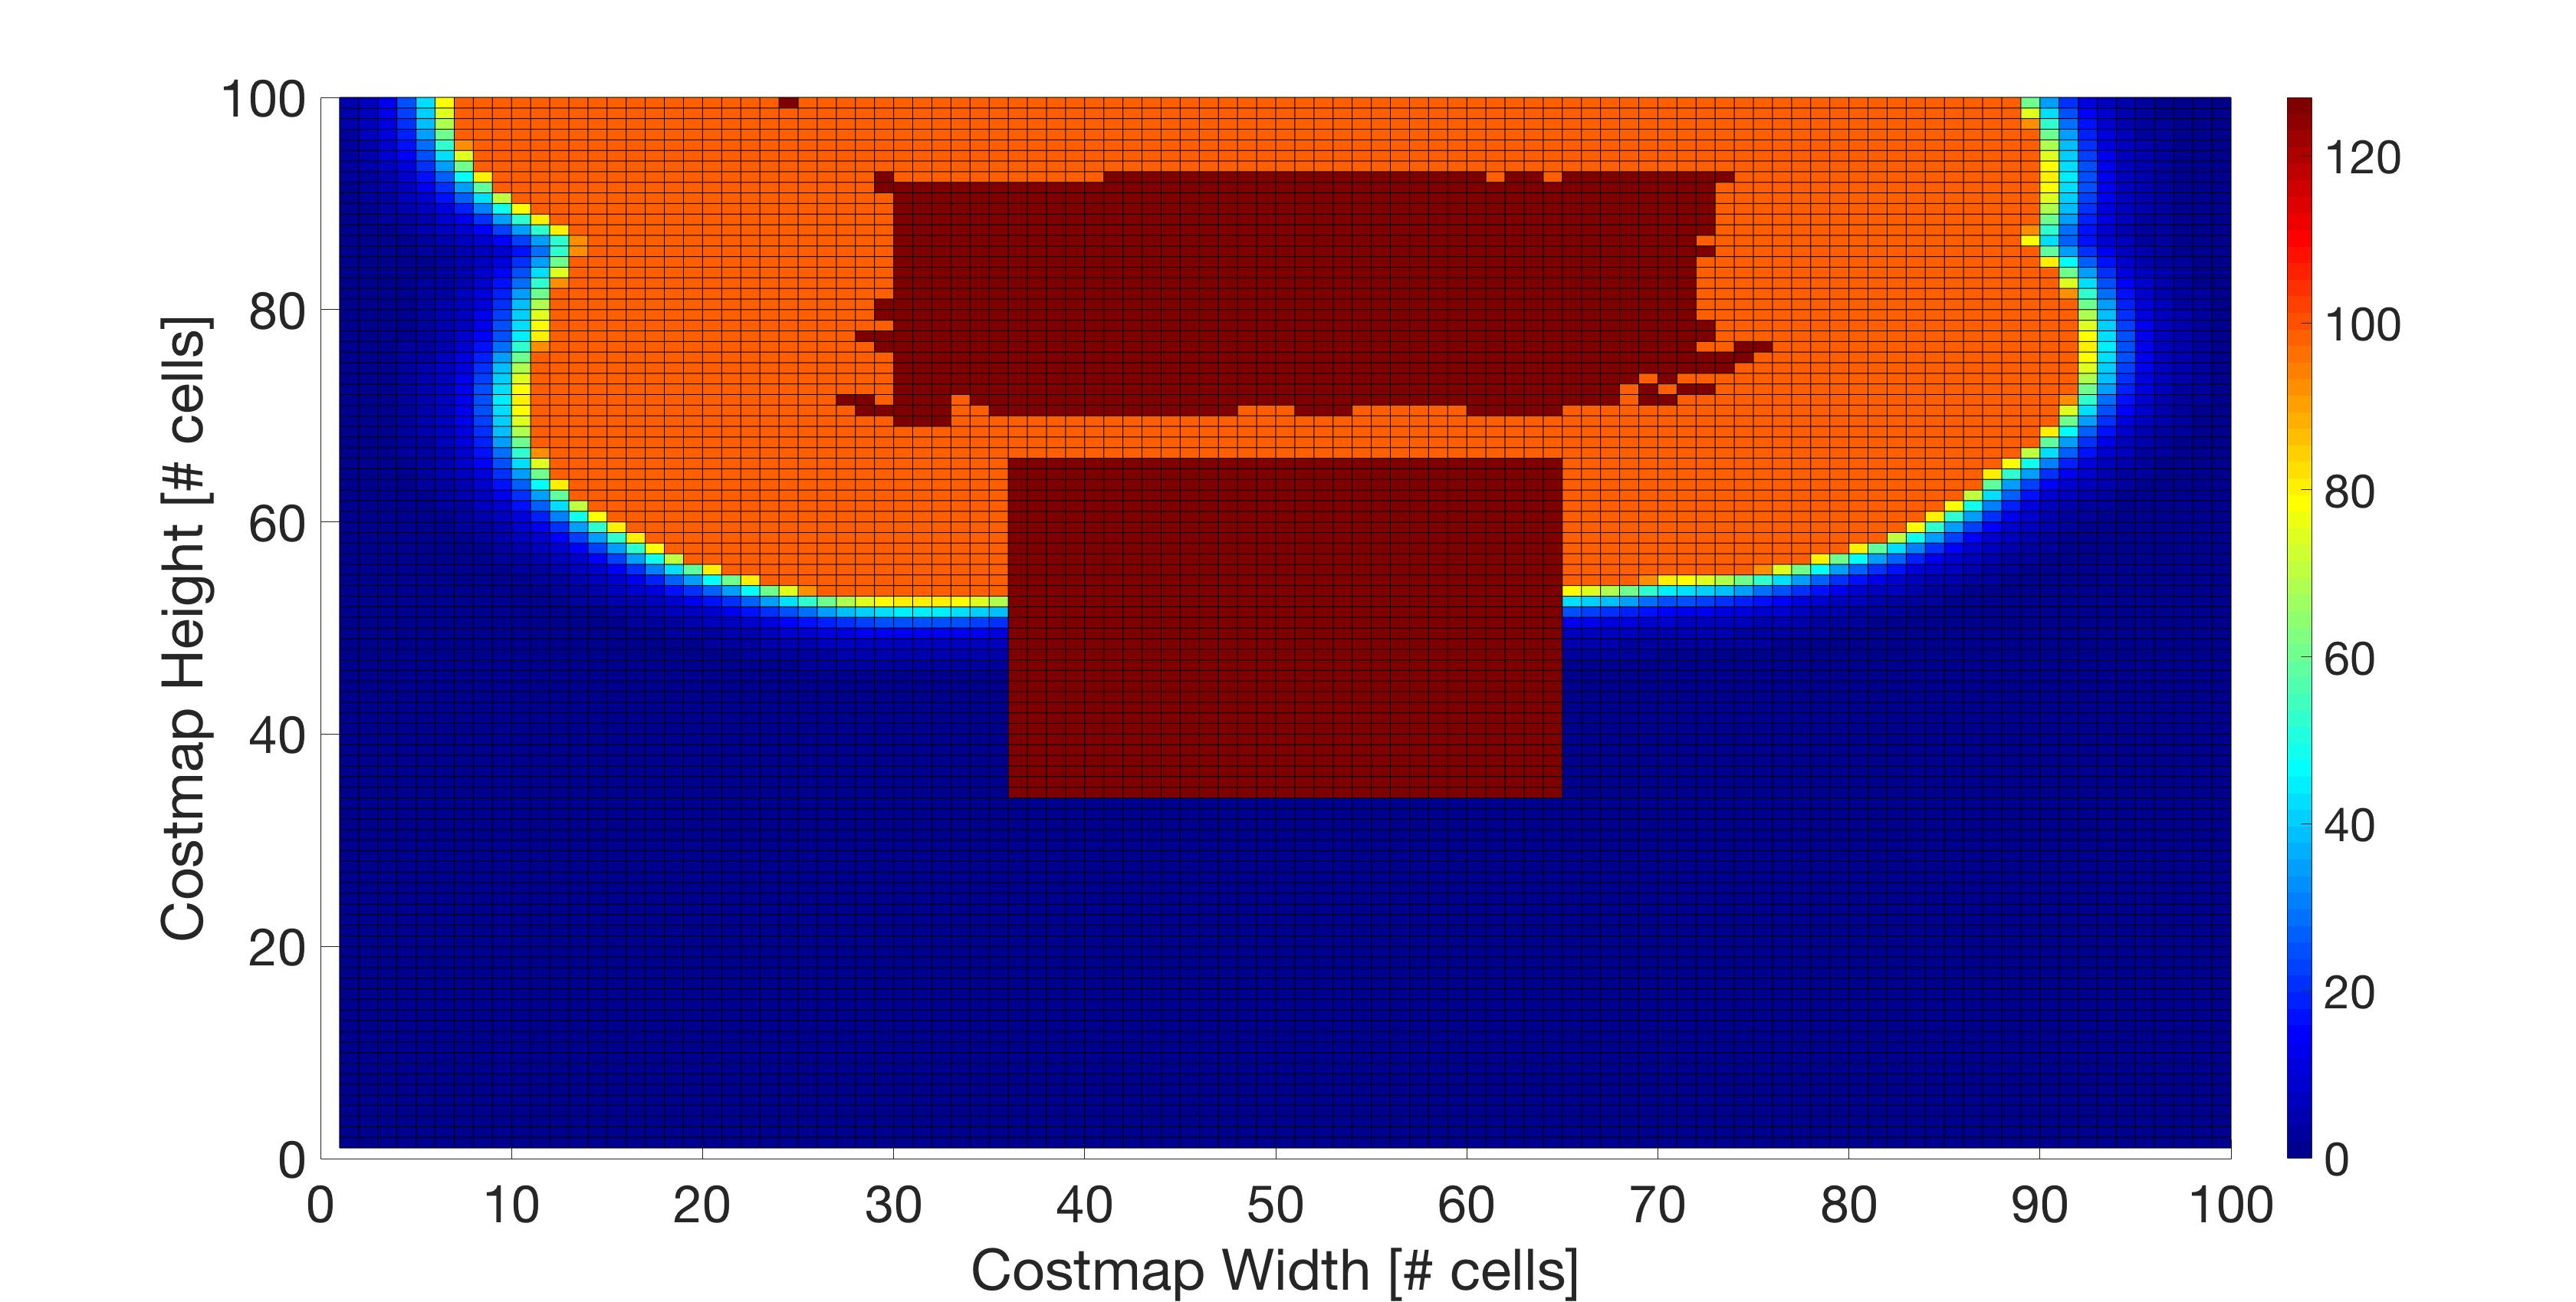
\includegraphics[width=0.75\textwidth]{images/test2_costmap.jpg}
   \caption{Costmap at \unit{34}{s} of the frontal test. Dark red indicate the obstacle and the robot base.}
   \label{pics:test2costmap}
\end{figure}



\subsection{Corridor}
\section{Real World Scenarios Performance}
\subsection{Corner}
\begin{figure}
   \centering
   \includegraphics[width=0.75\textwidth]{images/test16_setup2.jpg}
   \caption{Setup of the \unit{2}{m} wide corner scenario.}
   \label{pics:test16_setup}
\end{figure}

\begin{figure}
   \centering
   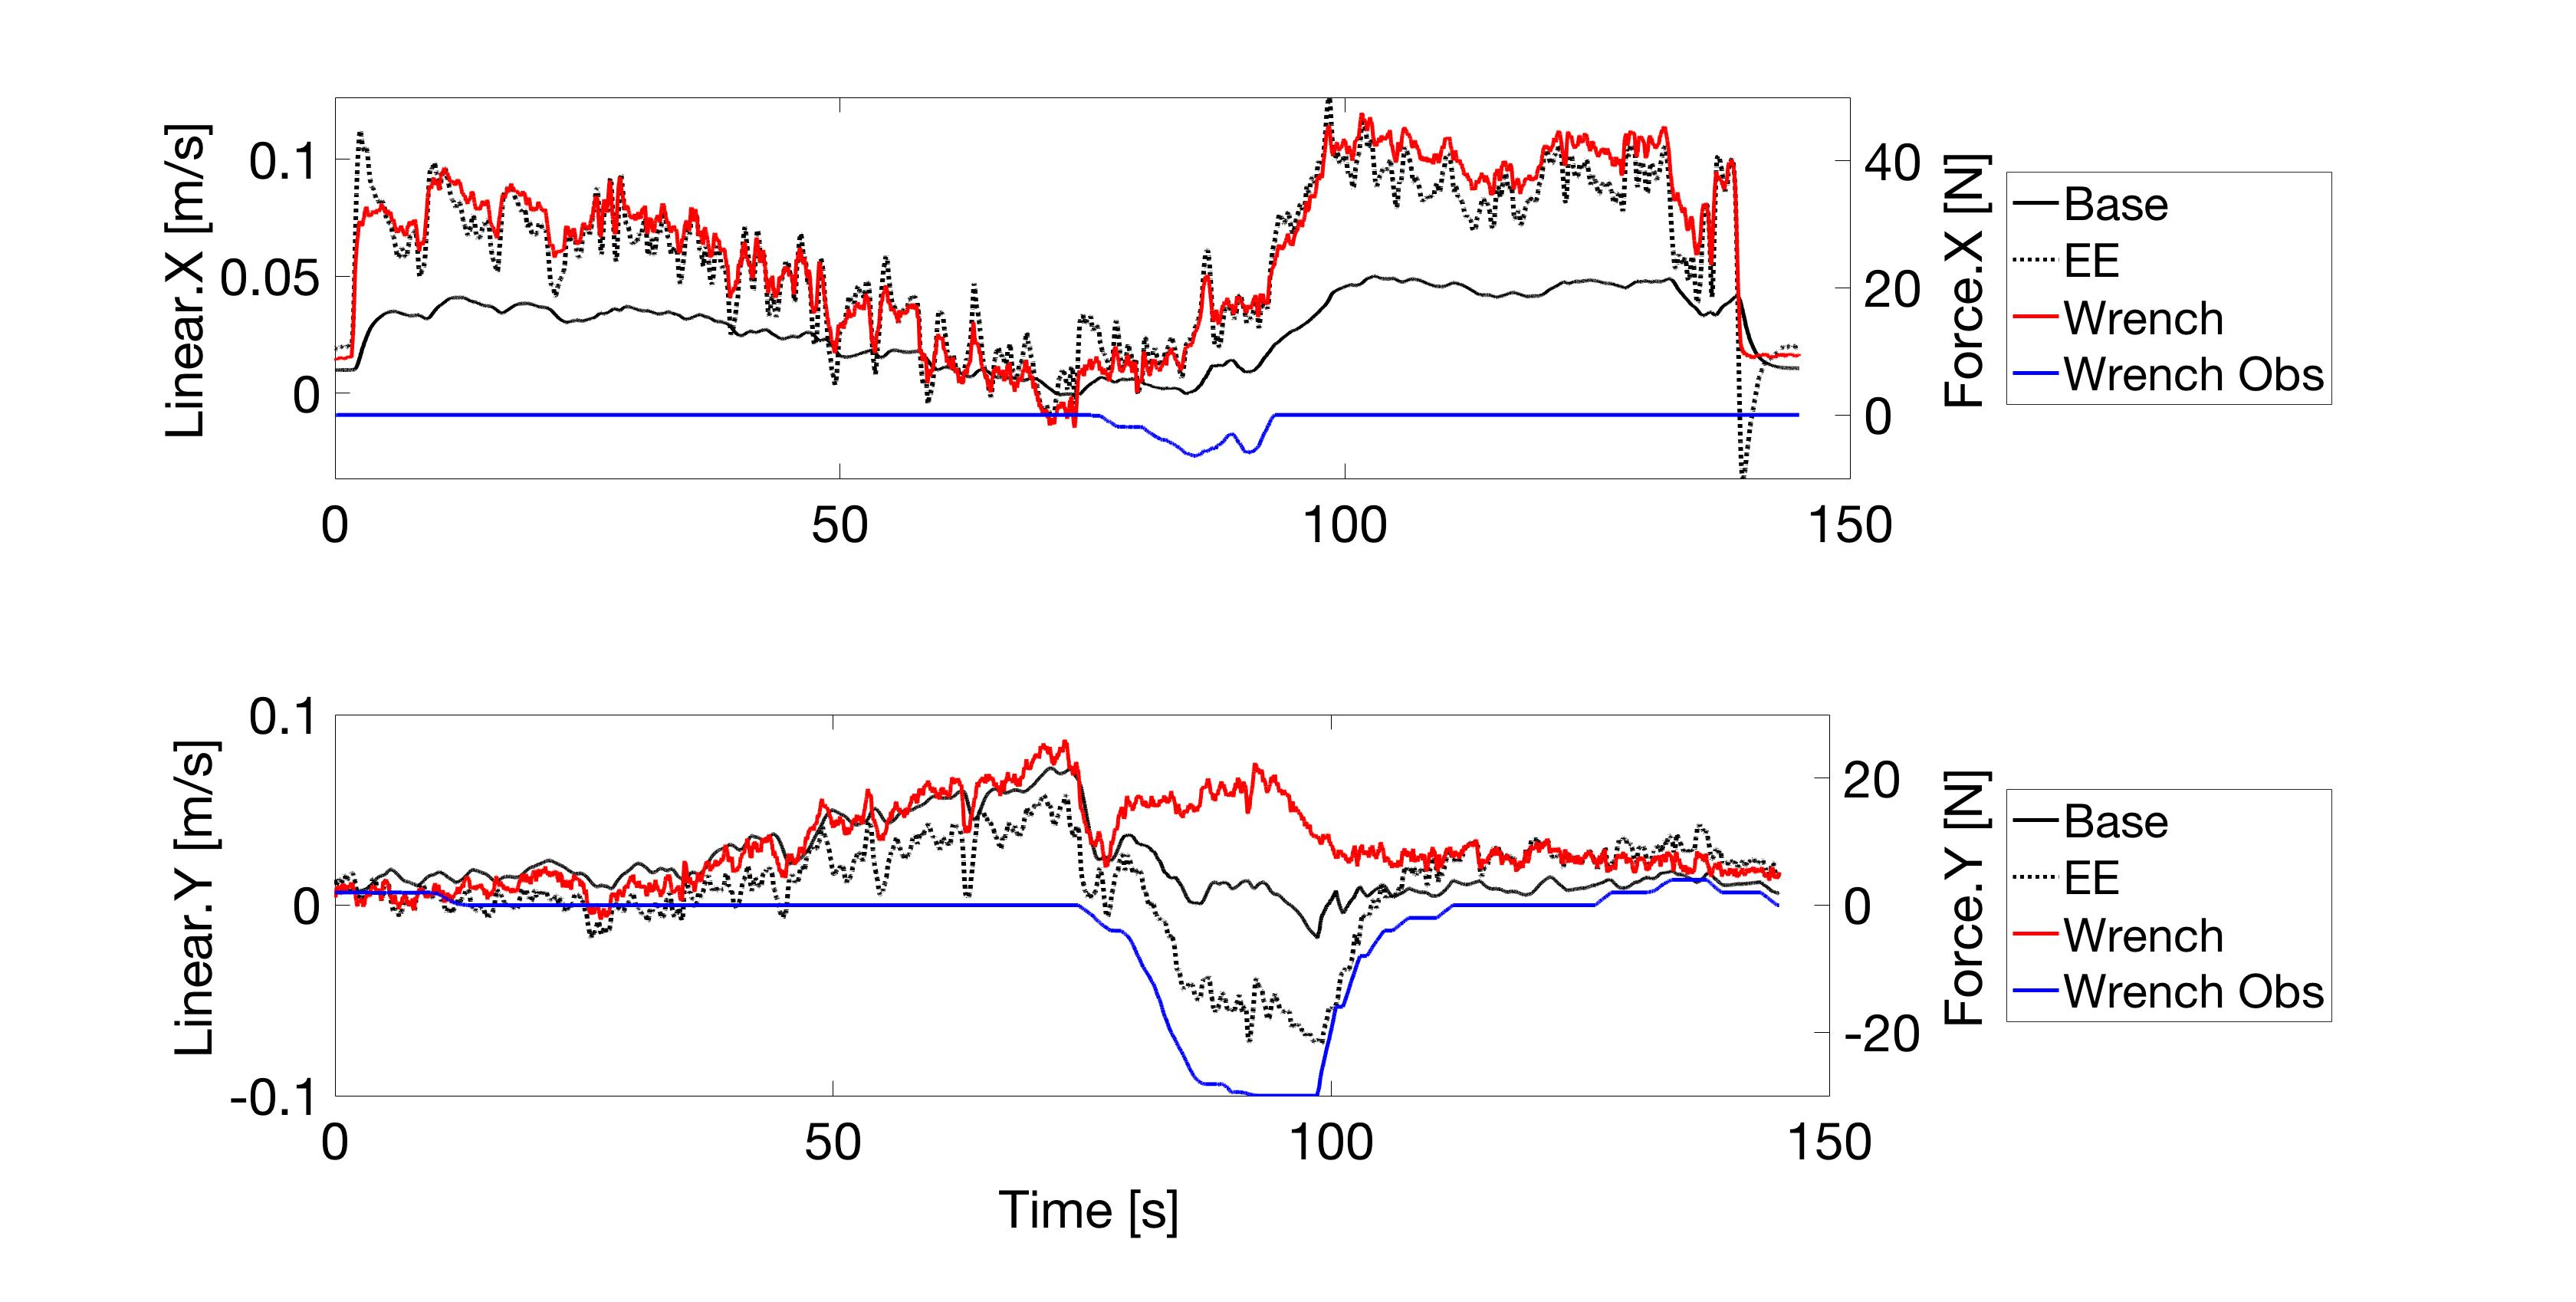
\includegraphics[width=0.75\textwidth]{images/test16.jpg}
   \caption{Velocity response to external and obstacle force input in \unit{2}{m} wide corner scenario.}
   \label{pics:test16}
\end{figure}

In this experiment, we asses the performance of the algorithm in a corrider with a corner. The width of corridor is \unit{2}{m} and we jointly carry the object through it. As we can see in \cref{pics:test16}, there is a negative peak in the negative $Y$
direction, which is caused by the robot drifting close the outer wall as it was making the corner. This was due to the fact, that

\subsection{Double Slalom}
\subsection{Triple Slalom}
\subsection{Cluttered Space 1}
\subsection{Cluttered Space 2}
\chapter{Conclusions}

\chapter{Einige wichtige Hinweise zum Arbeiten mit \LaTeX\ }
\label{sec:latexumg}

Nachfolgend wird die Codierung einiger oft verwendeten Elemente
kurz beschrieben. Das Einbinden von Bildern ist in \LaTeX\ nicht
ganz unproblematisch und hängt auch stark vom verwendeten Compiler
ab. Typisches Format für Bilder in \LaTeX\ ist
EPS\footnote{Encapsulated Postscript} oder PDF\footnote{Portable Document Format}.


\section{Gliederungen}
\label{sec:gliederung}

Ein Text kann mit den Befehlen \texttt{\textbackslash
chapter\{.\}}, \texttt{\textbackslash section\{.\}},
\texttt{\textbackslash subsection\{.\}} und \texttt{\textbackslash
subsubsection\{.\}} gegliedert werden.


\section{Referenzen und Verweise}
\label{sec:refverw}

Literaturreferenzen werden mit dem Befehl \texttt{\textbackslash
citep\{.\}} und \texttt{\textbackslash
citet\{.\}} erzeugt. Beispiele: ein Buch \citep{Raibert1986LeggedRobotsThatBalance}, ein Buch und ein Journal Paper \citep{Raibert1986LeggedRobotsThatBalance,Vukobratovic2004ZeroMomentPoint}, ein Konferenz Paper mit Erwähnung des Autors: \citet{Pratt1995SEA}.

Zur Erzeugung von Fussnoten wird der Befehl \texttt{\textbackslash
footnote\{.\}} verwendet. Auch hier ein Beispiel\footnote{Bla
bla.}.

Querverweise im Text werden mit \texttt{\textbackslash label\{.\}}
verankert und mit \texttt{\textbackslash cref\{.\}} erzeugt.
Beispiel einer Referenz auf das zweite Kapitel:
\cref{sec:latexumg}.


\section{Aufzählungen}\label{sec:aufz}

Folgendes Beispiel einer Aufzählung ohne Numerierung,
\begin{itemize}
  \item Punkt 1
  \item Punkt 2
\end{itemize}
wurde erzeugt mit:
\begin{verbatim}
\begin{itemize}
  \item Punkt 1
  \item Punkt 2
\end{itemize}
\end{verbatim}

Folgendes Beispiel einer Aufzählung mit Numerierung,
\begin{enumerate}
  \item Punkt 1
  \item Punkt 2
\end{enumerate}
wurde erzeugt mit:
\begin{verbatim}
\begin{enumerate}
  \item Punkt 1
  \item Punkt 2
\end{enumerate}
\end{verbatim}

Folgendes Beispiel einer Auflistung,
\begin{description}
  \item[P1] Punkt 1
  \item[P2] Punkt 2
\end{description}
wurde erzeugt mit:
\begin{verbatim}
\begin{description}
  \item[P1] Punkt 1
  \item[P2] Punkt 2
\end{description}
\end{verbatim}


\section{Erstellen einer Tabelle}\label{sec:tabellen}

Ein Beispiel einer Tabelle:
\begin{table}[h]
\begin{center}
 \caption{Daten der Fahrzyklen ECE, EUDC, NEFZ.}\vspace{1ex}
 \label{tab:tabnefz}
 \begin{tabular}{ll|ccc}
 \hline
 Kennzahl & Einheit & ECE & EUDC & NEFZ \\ \hline \hline
 Dauer & s & 780 & 400 & 1180 \\
 Distanz & km & 4.052 & 6.955 & 11.007 \\
 Durchschnittsgeschwindigkeit & km/h & 18.7 &  62.6 & 33.6 \\
 Leerlaufanteil & \% & 36 & 10 & 27 \\
 \hline
 \end{tabular}
\end{center}
\end{table}

Die Tabelle wurde erzeugt mit:
\begin{verbatim}
\begin{table}[h]
\begin{center}
 \caption{Daten der Fahrzyklen ECE, EUDC, NEFZ.}\vspace{1ex}
 \label{tab:tabnefz}
 \begin{tabular}{ll|ccc}
 \hline
 Kennzahl & Einheit & ECE & EUDC & NEFZ \\ \hline \hline
 Dauer & s & 780 & 400 & 1180 \\
 Distanz & km & 4.052 & 6.955 & 11.007 \\
 Durchschnittsgeschwindigkeit & km/h & 18.7 &  62.6 & 33.6 \\
 Leerlaufanteil & \% & 36 & 10 & 27 \\
 \hline
 \end{tabular}
\end{center}
\end{table}
\end{verbatim}


\section{Einbinden einer Grafik}\label{sec:epsgraph}

Das Einbinden von Graphiken kann wie folgt bewerkstelligt werden:
\begin{verbatim}
\begin{figure}
   \centering
   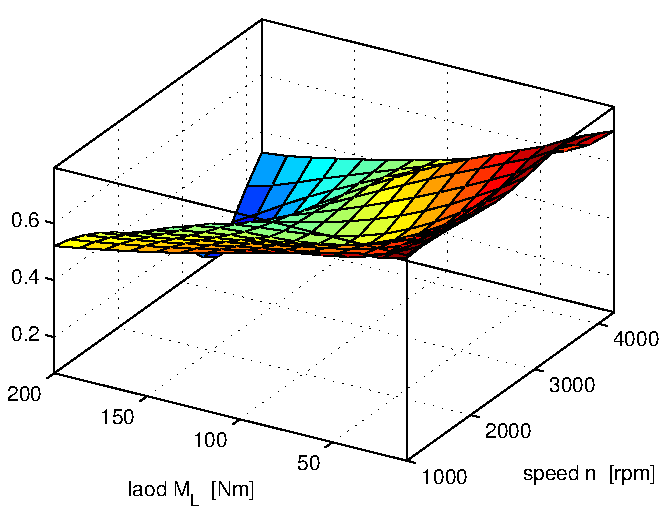
\includegraphics[width=0.75\textwidth]{images/k_surf.pdf}
   \caption{Ein Bild.}
   \label{fig:k_surf}
\end{figure}
\end{verbatim}

\begin{figure}
   \centering
   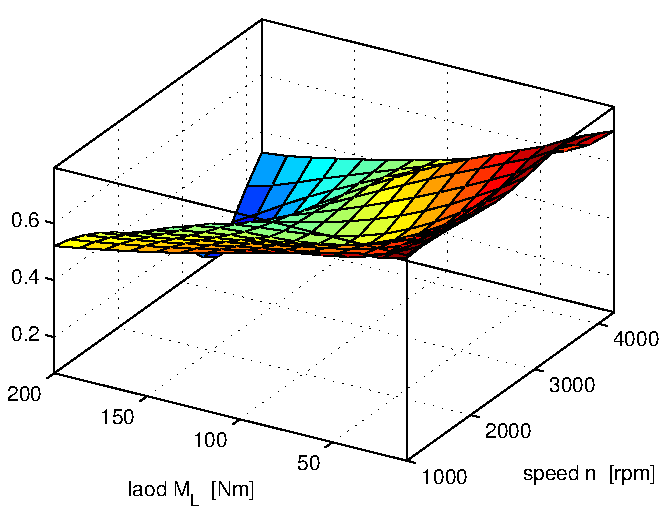
\includegraphics[width=0.75\textwidth]{images/k_surf.pdf}
   \caption{Ein Bild}
   \label{pics:k_surf}
\end{figure}

oder bei zwei Bildern nebeneinander mit:
\begin{verbatim}
\begin{figure}
  \begin{minipage}[t]{0.48\textwidth}
    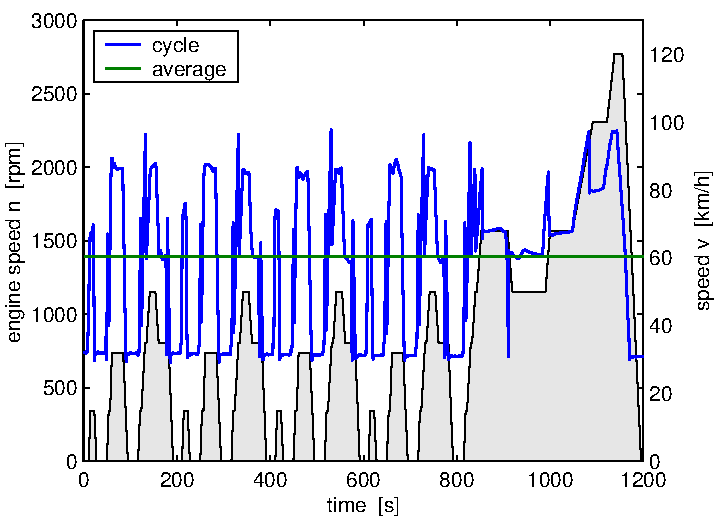
\includegraphics[width = \textwidth]{images/cycle_we.pdf}
  \end{minipage}
  \hfill
  \begin{minipage}[t]{0.48\textwidth}
    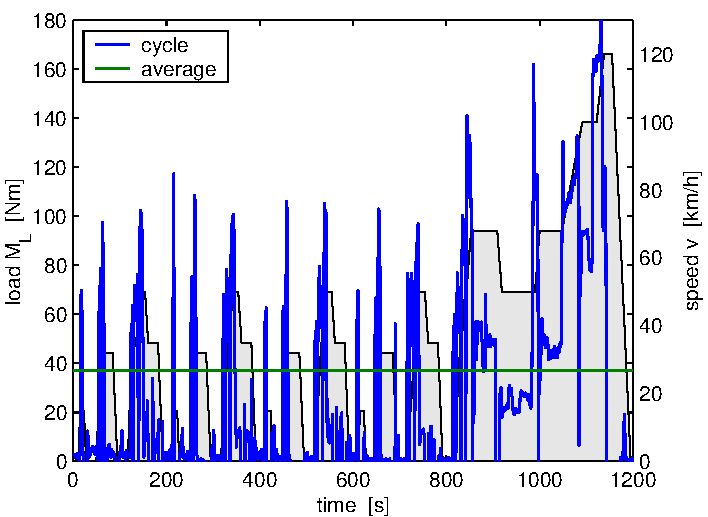
\includegraphics[width = \textwidth]{images/cycle_ml.pdf}
  \end{minipage}
  \caption{Zwei Bilder nebeneinander.}
  \label{pics:cycle}
\end{figure}
\end{verbatim}

\begin{figure}
  \begin{minipage}[t]{0.48\textwidth}
    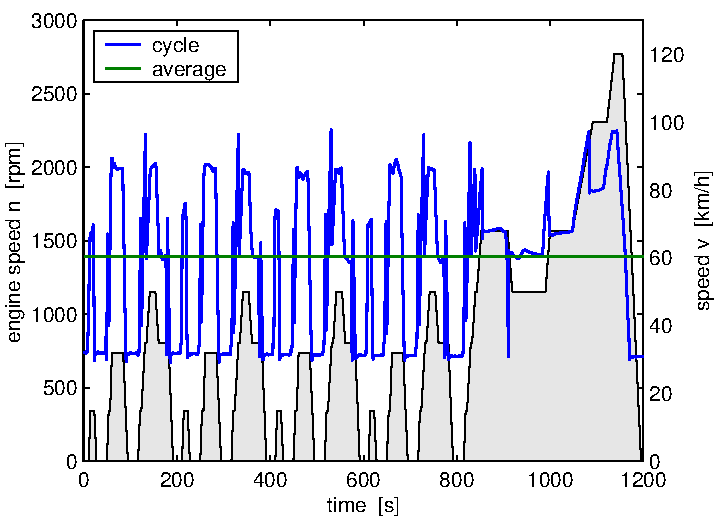
\includegraphics[width = \textwidth]{images/cycle_we.pdf}
  \end{minipage}
  \hfill
  \begin{minipage}[t]{0.48\textwidth}
    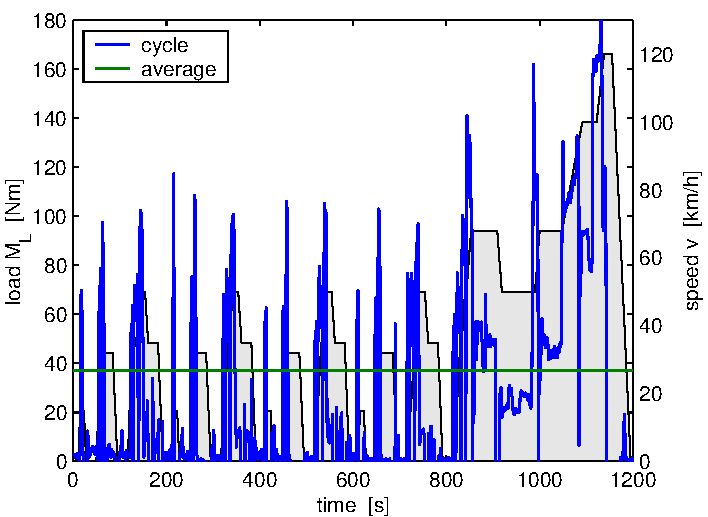
\includegraphics[width = \textwidth]{images/cycle_ml.pdf}
  \end{minipage}
  \caption{Zwei Bilder nebeneinander}
  \label{pics:cycle}
\end{figure}


\section{Mathematische Formeln}\label{sec:math}

Einfache mathematische Formeln werden mit der equation-Umgebung
erzeugt:
\begin{equation}
 p_{me0f}(T_e,\omega_e) \ = \ k_1(T_e) \cdot (k_2+k_3 S^2
 \omega_e^2) \cdot \Pi_{\mathrm{max}} \cdot \sqrt{\frac{k_4}{B}} \, .
 	\label{eq:my_equation}
\end{equation}

Der Code dazu lautet:
\begin{verbatim}
\begin{equation}
 p_{me0f}(T_e,\omega_e) \ = \ k_1(T_e) \cdot (k_2+k_3 S^2
 \omega_e^2) \cdot \Pi_{max} \cdot \sqrt{\frac{k_4}{B}} \, .
\end{equation}
\end{verbatim}

Mathematische Ausdrücke im Text werden mit \$formel\$ erzeugt (z.B.:
$a^2+b^2=c^2$).

Vektoren und Matrizen werden mit den Befehlen \texttt{\textbackslash vec\{.\}} und \texttt{\textbackslash mat\{.\}} erzeugt (z.B. $\vec{v}$, $\mat{M}$).


\section{Weitere nützliche Befehle}\label{sec:div}

Hervorhebungen im Text sehen so aus: \emph{hervorgehoben}. Erzeugt
werden sie mit dem \texttt{\textbackslash epmh\{.\}} Befehl.

Einheiten werden mit den Befehlen \texttt{\textbackslash unit[1]\{m\}} (z.B.~\unit[1]{m}) und \texttt{\textbackslash unitfrac[1]\{m\}\{s\}} (z.B.~\unitfrac[1]{m}{s}) gesetzt.
